\documentclass[12pt,addpoints]{repaso}
\grado{2}
\nivel{Secundaria}
\cicloescolar{2023-2024}
\materia{Matemáticas}
\unidad{2}
\title{Practica la Unidad}
\aprendizajes{
    \item Formula expresiones de primer grado para representar propiedades (perímetros y áreas) de figuras geométricas y verifica equivalencia de expresiones, tanto algebraica como geométricamente (análisis de las figuras).
    \item Construye polígonos regulares a partir de algunas medidas (lados, apotema, diagonales, etcétera).
    \item Descompone figuras en otras para calcular su área.
    \item Calcula el perímetro y el área de polígonos regulares y del círculo a partir de diferentes datos.
}
\author{Melchor Pinto, J.C.}
\begin{document}
\INFO%
\begin{multicols}{2}
    \include*{../blocks/block002}
    \include*{../blocks/block035c}
    \include*{../blocks/block003}
    \include*{../blocks/block035b}
\end{multicols}
\newpage
\section*{Círculo}
\subsection*{Resolución de problemas}
\begin{questions}
    \questionboxed[4]{Resuelve los siguientes problemas:
        \begin{multicols}{2}
            \begin{parts}
                \part Una casa tiene una alberca circular de 6 metros de diámetro. Calcula el área de la alberca.
                \fillin[$28.26$ m$^2$][0in]
                \part El radio de una rueda es de 32 centímetros, ¿cuántos centímetros habrá recorrido esa rueda después de haber dado 22 vueltas?
                \fillin[$70737.92$ cm][0in]

                \columnbreak

                \part Calcula el área de un parque que tiene un radio de 170 metros.
                \fillin[$90746$ m][0in]
                \part Daniel tiene un terreno circular con un radio de 6 metros al cual le desea poner una barda en su periferia, si el precio por metro de barda es de 124 pesos. ¿Cuánto pagará en total por poner la barda?
                \fillin[$\$4,672.32$ pesos][0in]
            \end{parts}
        \end{multicols}
    }

    \subsection*{Radio, Diámetro, Perímetro y Área de un círculo}
    \questionboxed[6]{Encuentra el perímetro y el área de los siguientes círculos:
        \begin{multicols}{3}
            \begin{parts}
                \part 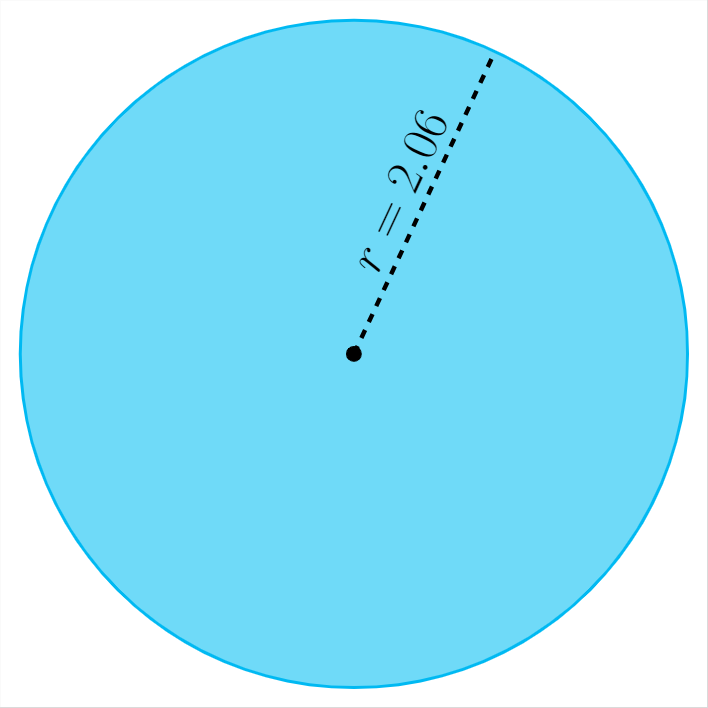
\includegraphics[width=0.85\linewidth]{mex_0001.png}\\
                Perímetro: \fillin[][0.3in] \quad Área: \fillin[][0.3in]
                \part 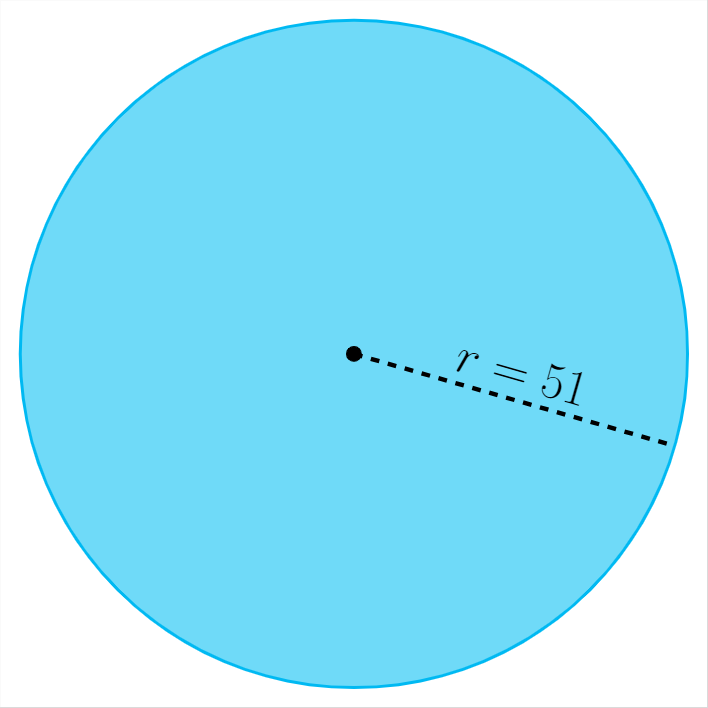
\includegraphics[width=0.85\linewidth]{mex_0002.png}\\
                Perímetro: \fillin[][0.3in] \quad Área: \fillin[][0.3in]
                % \part 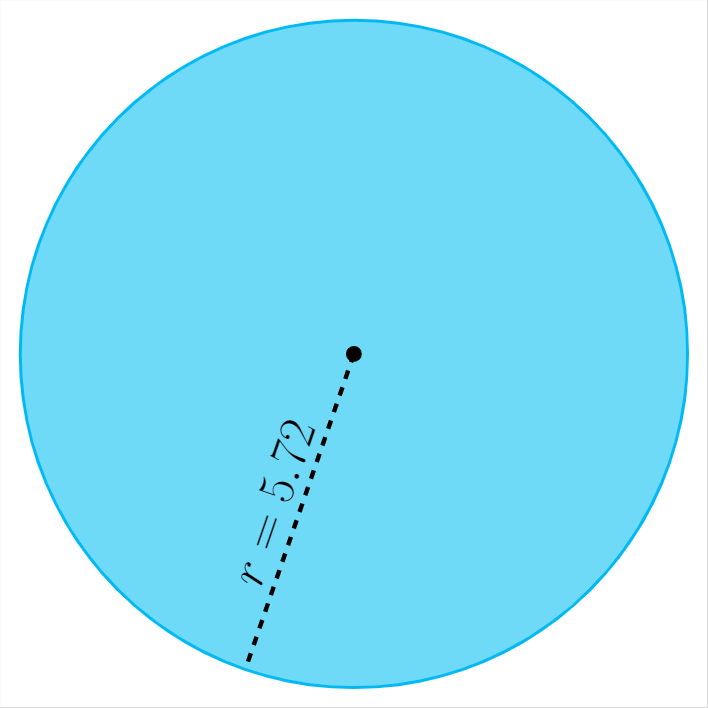
\includegraphics[width=0.85\linewidth]{mex_0003.png}\\
                % Perímetro: \fillin[][0.3in] \quad Área: \fillin[][0.3in]
                % \part 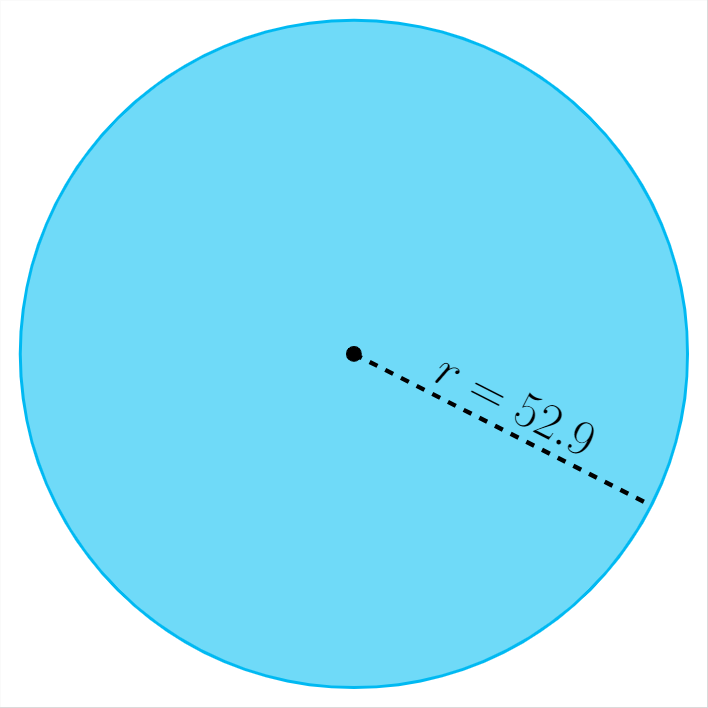
\includegraphics[width=0.85\linewidth]{mex_0004.png}\\
                % Perímetro: \fillin[][0.3in] \quad Área: \fillin[][0.3in]
                \part 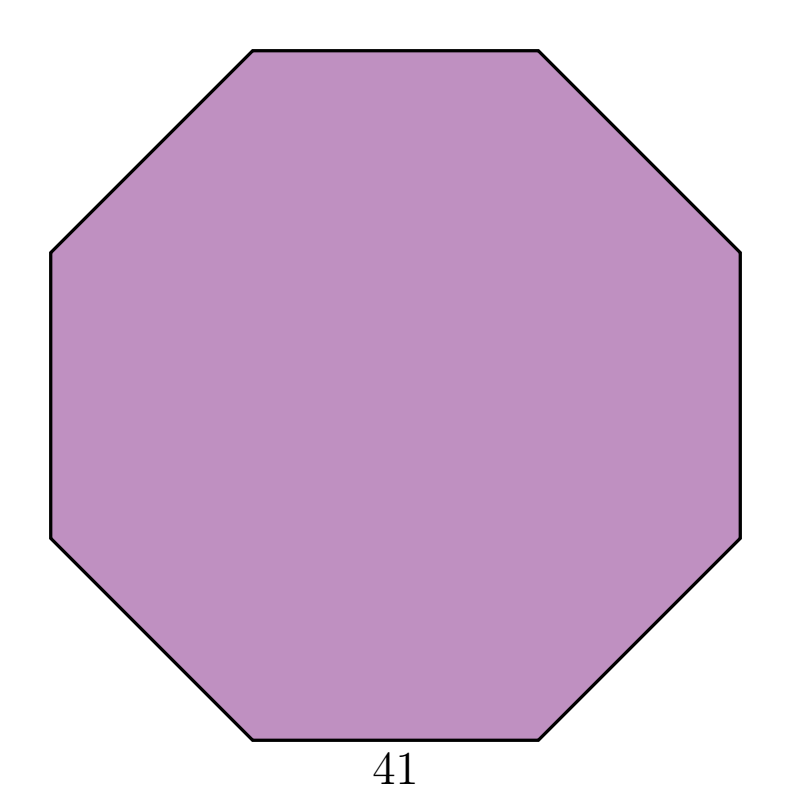
\includegraphics[width=0.85\linewidth]{mex_0005.png}\\
                Perímetro: \fillin[][0.3in] \quad Área: \fillin[][0.3in]
                % \part 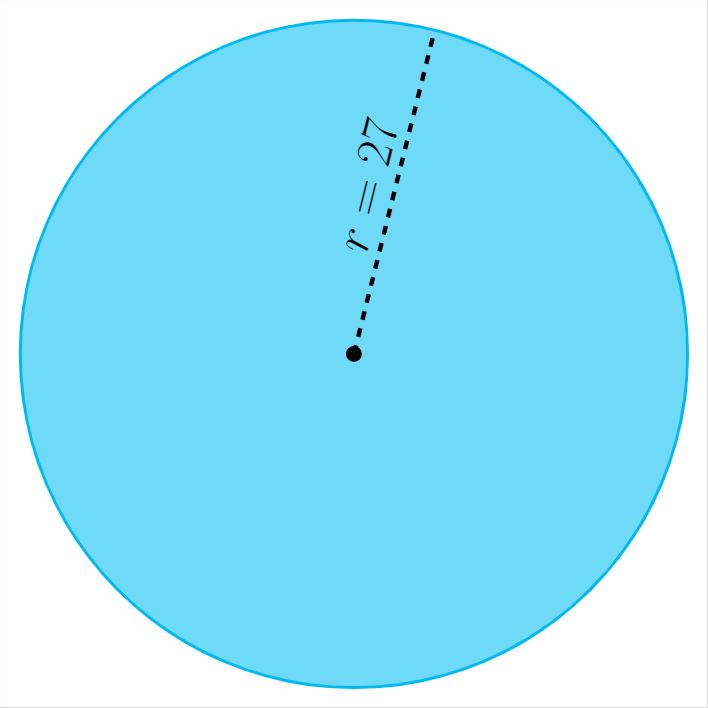
\includegraphics[width=0.85\linewidth]{mex_0006.png}\\
                % Perímetro: \fillin[][0.3in] \quad Área: \fillin[][0.3in]
                \part 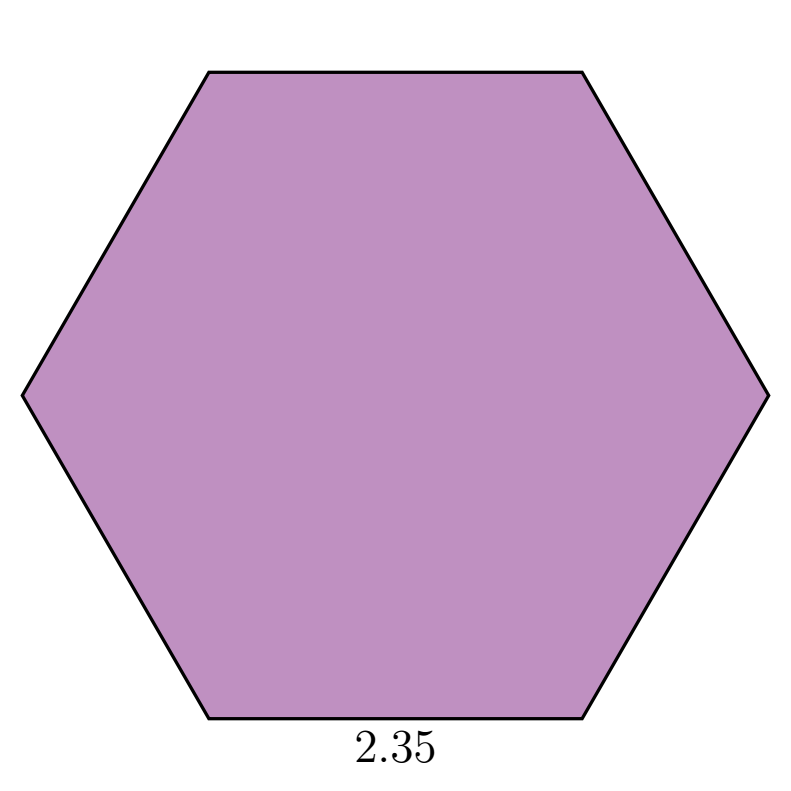
\includegraphics[width=0.85\linewidth]{mex_0007.png}\\
                Perímetro: \fillin[][0.3in] \quad Área: \fillin[][0.3in]
                \part 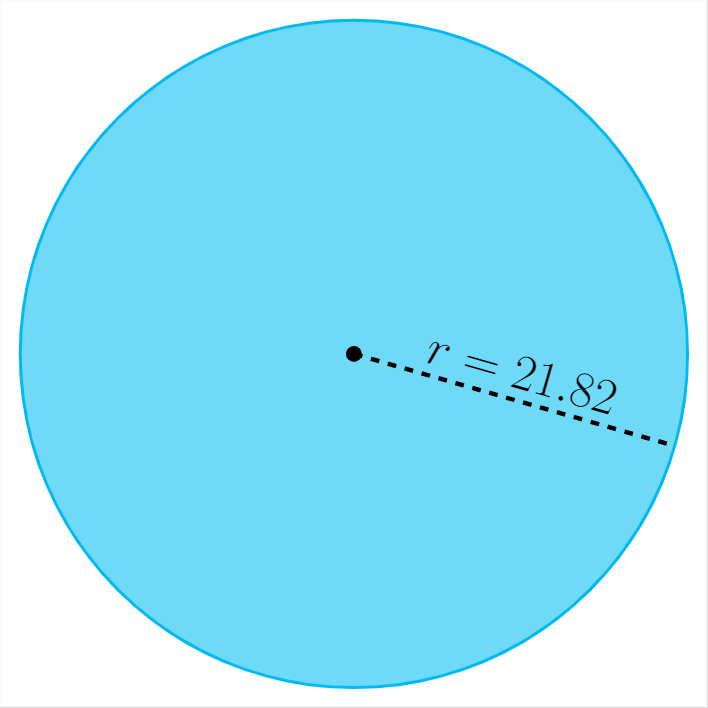
\includegraphics[width=0.85\linewidth]{mex_0008.png}\\
                Perímetro: \fillin[][0.3in] \quad Área: \fillin[][0.3in]
                \part 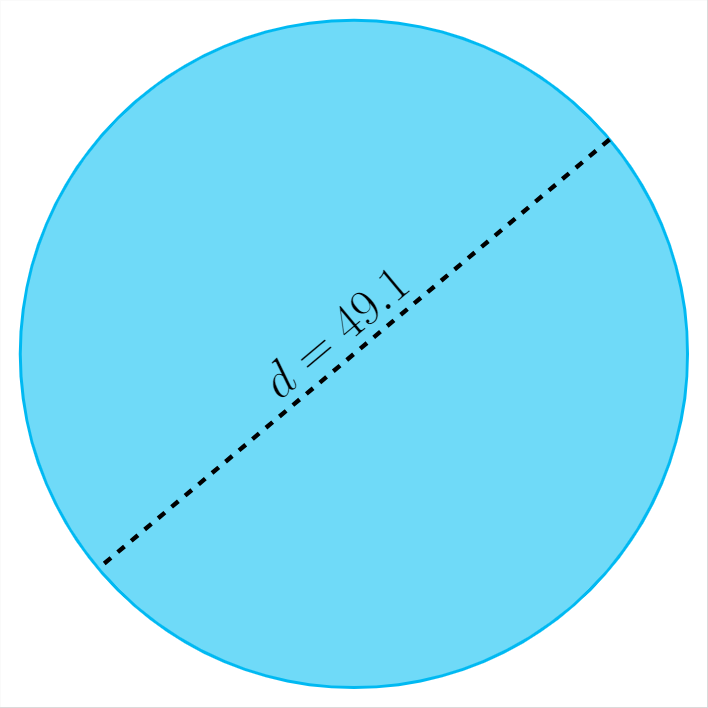
\includegraphics[width=0.85\linewidth]{mex_0009.png}\\
                Perímetro: \fillin[][0.3in] \quad Área: \fillin[][0.3in]
                % \part 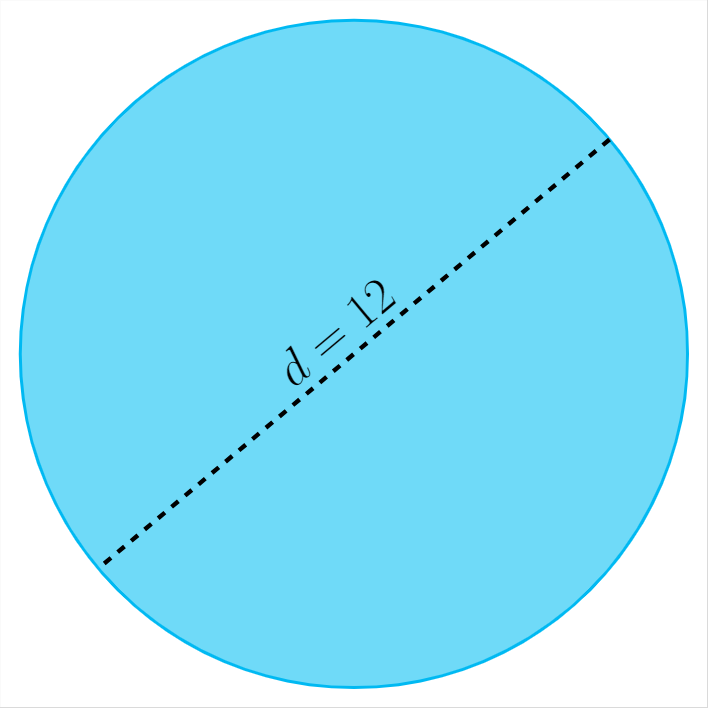
\includegraphics[width=0.85\linewidth]{mex_0010.png}\\
                % Perímetro: \fillin[][0.3in] \quad Área: \fillin[][0.3in]
                % \part 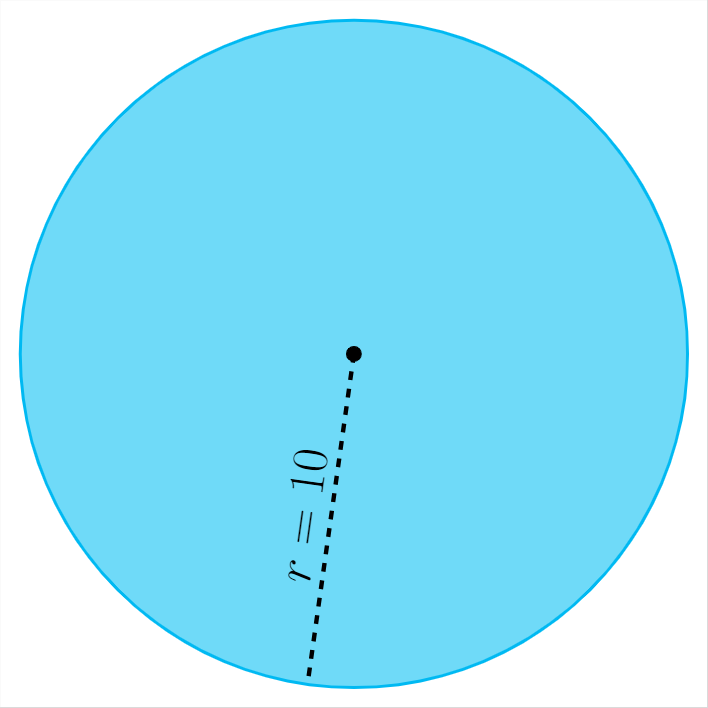
\includegraphics[width=0.85\linewidth]{mex_0011.png}\\
                % Perímetro: \fillin[][0.3in] \quad Área: \fillin[][0.3in]
                % \part 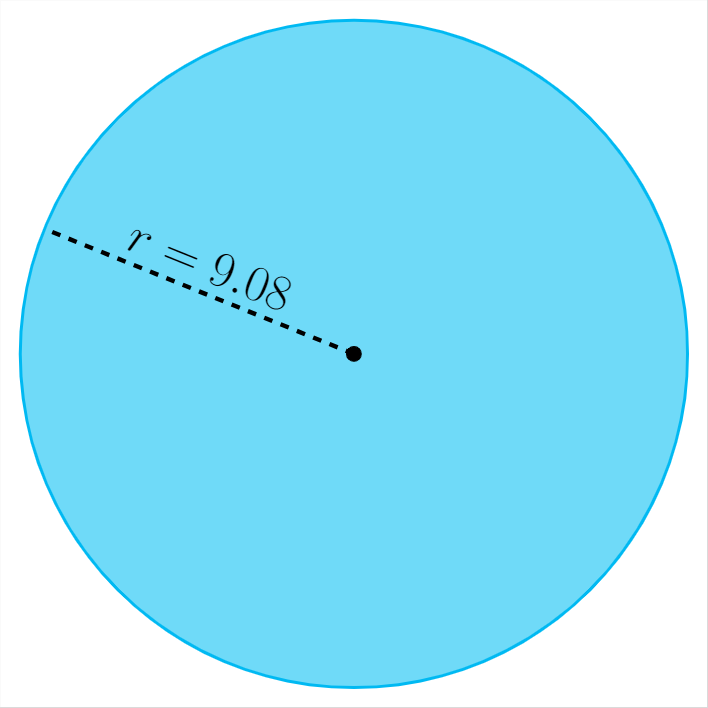
\includegraphics[width=0.85\linewidth]{mex_0012.png}\\
                % Perímetro: \fillin[][0.3in] \quad Área: \fillin[][0.3in]
            \end{parts}
        \end{multicols}
    }

    \newpage
    \section*{Polígonos y circunferencias}
    \subsection*{Ángulos interiores}

    \questionboxed[4]{Responde a las siguientes preguntas:
        \begin{multicols}{2}
            \begin{parts}
                % \part ¿Cuánto mide el ángulo interior de un hexágono regular? \fillin[$120$][0in]

                % \begin{solutionbox}{2cm}
                % \end{solutionbox}

                % \part ¿Cuánto mide el ángulo interior de un pentadecágono regular? \fillin[$156$][0in]

                % \begin{solutionbox}{2cm}
                % \end{solutionbox}

                \part La suma de los ángulos interiores de un polígono de 8 lados es: \fillin[$1080$][0in]

                \begin{solutionbox}{2cm}
                \end{solutionbox}

                \part ¿Cuánto mide el ángulo interior de un dodecágono regular? \fillin[$150$][0in]

                \begin{solutionbox}{2cm}
                \end{solutionbox}

                \part La suma de los ángulos interiores de un polígono de 11 lados es: \fillin[$1620$][0in]

                \begin{solutionbox}{2cm}
                \end{solutionbox}

                \part ¿Cuánto mide el ángulo interior de un icoságono regular? \fillin[$162$][0in]

                \begin{solutionbox}{2cm}
                \end{solutionbox}

            \end{parts}
        \end{multicols}
    }

    \subsection*{Ángulos centrales y exteriores}

    \questionboxed[4]{Responde a las siguientes preguntas:
        \begin{multicols}{2}
            \begin{parts}
                \part ¿Cuánto mide el ángulo central de un polígono de 9 lados? \fillin[$40$][0in]

                \begin{solutionbox}{2cm}
                \end{solutionbox}

                \part ¿Cuánto mide el ángulo exterior de un polígono de 10 lados? \fillin[$36$][0in]

                \begin{solutionbox}{2cm}
                \end{solutionbox}

                % \part ¿Cuánto mide el ángulo central de un polígono de 15 lados? \fillin[$24$][0in]

                % \begin{solutionbox}{2cm}
                % \end{solutionbox}

                % \part ¿Cuánto mide el ángulo central de un polígono de 12 lados? \fillin[$30$][0in]

                % \begin{solutionbox}{2cm}
                % \end{solutionbox}

                \part ¿Cuánto mide el ángulo exterior de un polígono de 6 lados? \fillin[$60$][0in]

                \begin{solutionbox}{2cm}
                \end{solutionbox}

                \part ¿Cuánto mide el ángulo central de un polígono de 20 lados? \fillin[$18$][0in]

                \begin{solutionbox}{2cm}
                \end{solutionbox}

            \end{parts}
        \end{multicols}
    }
    \subsection*{Ángulos centrales e inscritos}

    \questionboxed[6]{Calcula el valor del ángulo $x$:
        \begin{multicols}{2}
            \begin{parts}
                \part 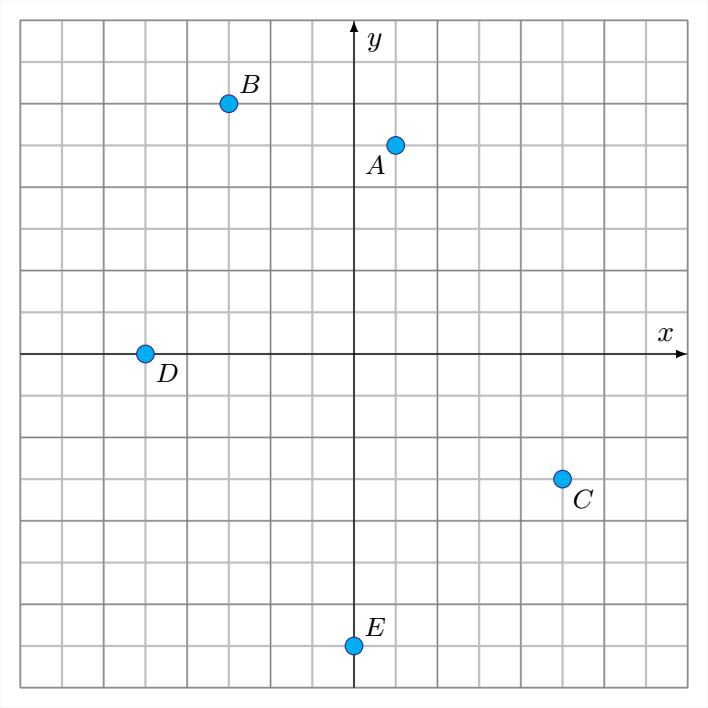
\includegraphics[width=0.7\linewidth]{mex_0043.png}\\
                $x=$ \fillin[$$ u][0.4in]

                \part 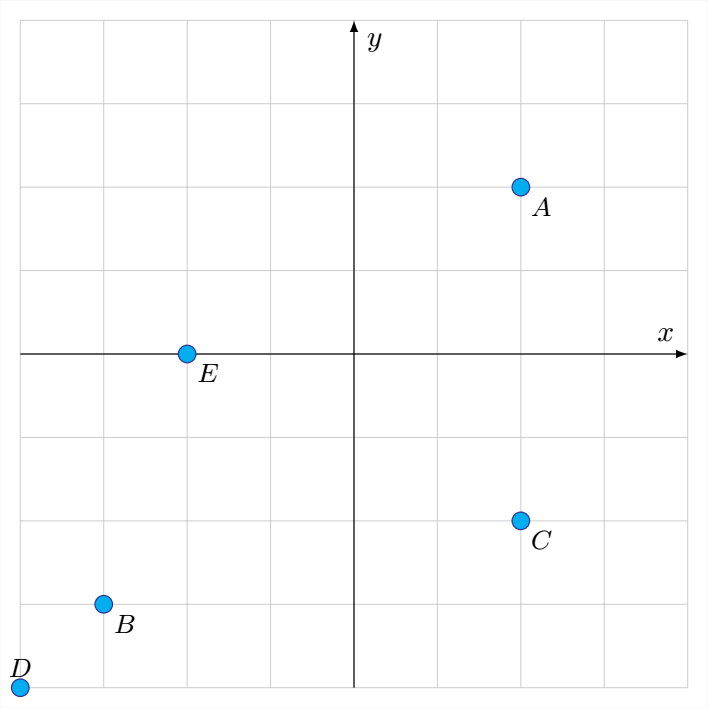
\includegraphics[width=0.7\linewidth]{mex_0044.png}\\
                $x=$ \fillin[$$ u][0.4in]

                \part 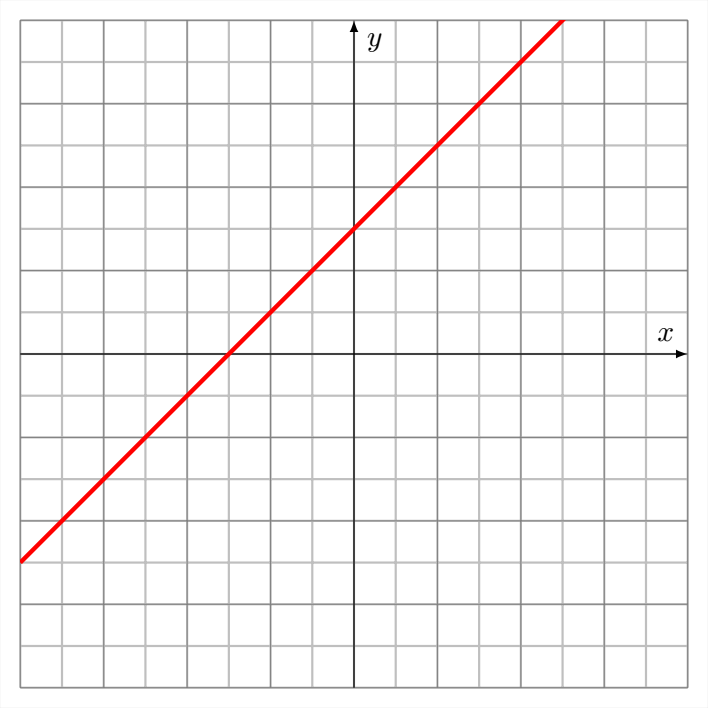
\includegraphics[width=0.7\linewidth]{mex_0046.png}\\
                $x=$ \fillin[$$ u][0.4in]

                \part 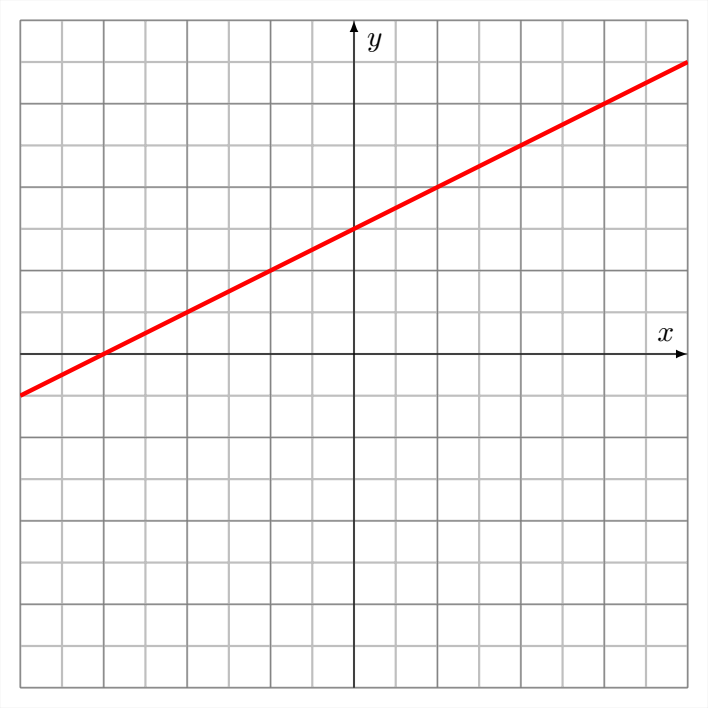
\includegraphics[width=0.7\linewidth]{mex_0047.png}\\
                $x=$ \fillin[$$ u][0.4in]

                \part 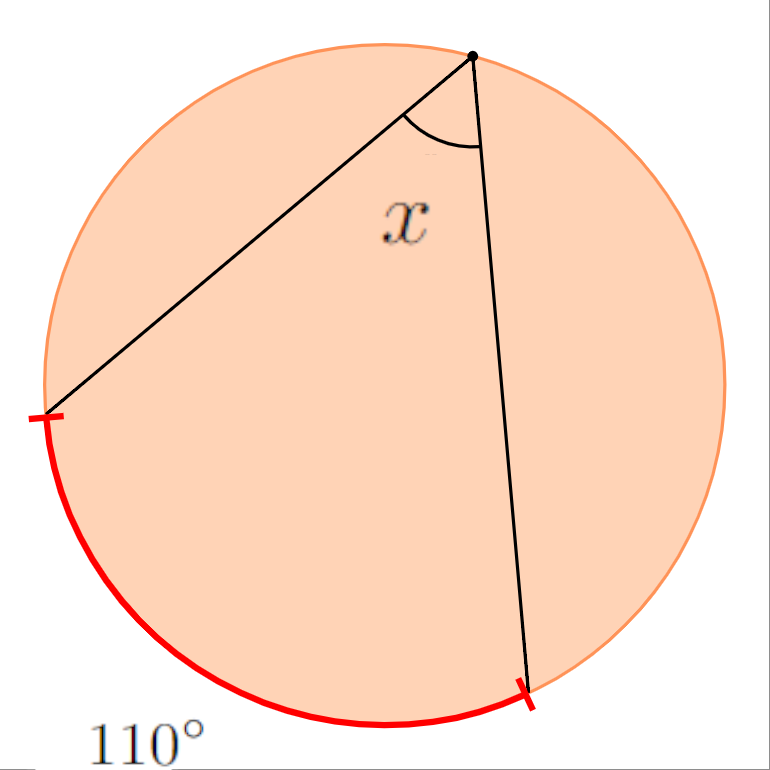
\includegraphics[width=0.7\linewidth]{mex_0049.png}\\
                $x=$ \fillin[$$ u][0.4in]

                \part 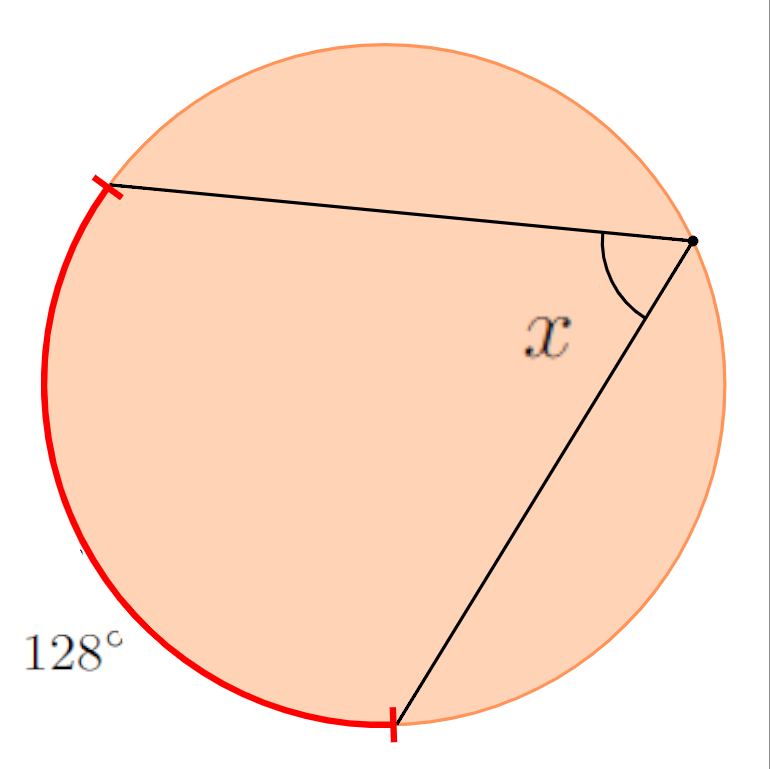
\includegraphics[width=0.7\linewidth]{mex_0050.png}\\
                $x=$ \fillin[$$ u][0.4in]
            \end{parts}
        \end{multicols}
    }

    \subsection*{Arco de una circunferencia}

    \questionboxed[6]{Calcula el valor del arco $x$:
        \begin{multicols}{2}
            \begin{parts}
                \part 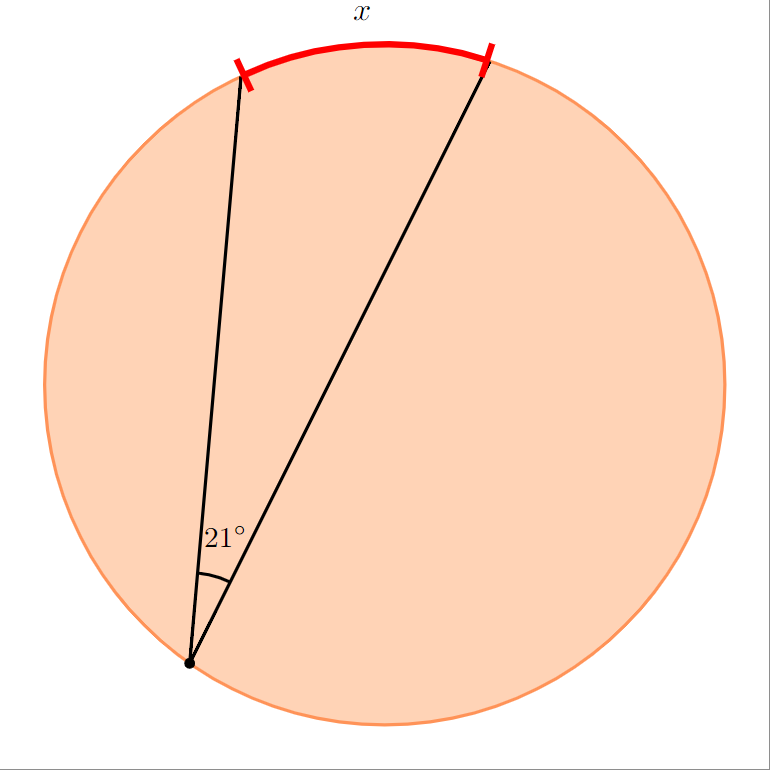
\includegraphics[width=0.7\linewidth]{mex_0052.png}\\
                $x=$ \fillin[$$ u][0.4in]

                \part 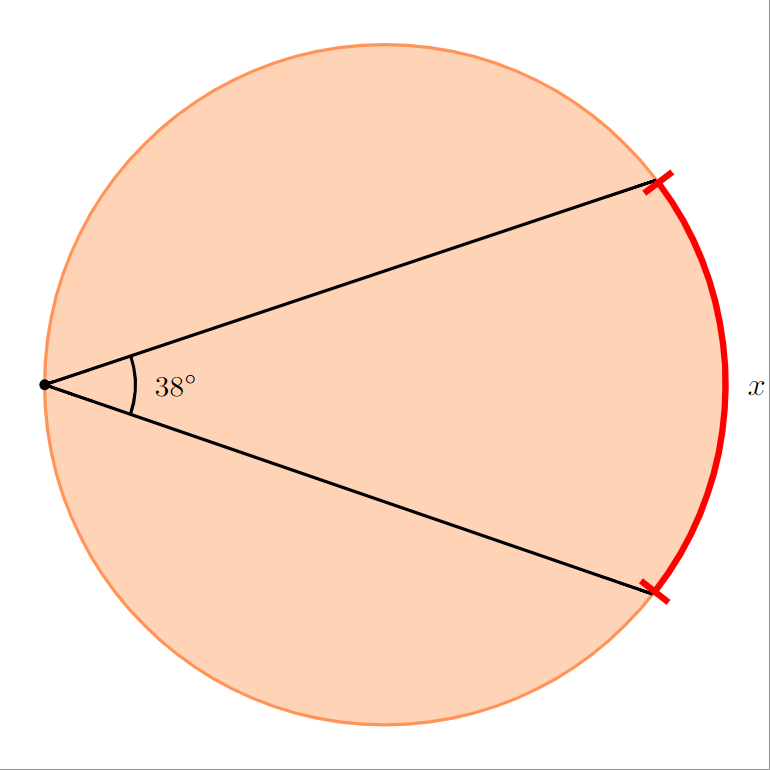
\includegraphics[width=0.7\linewidth]{mex_0053.png}\\
                $x=$ \fillin[$$ u][0.4in]

                \part 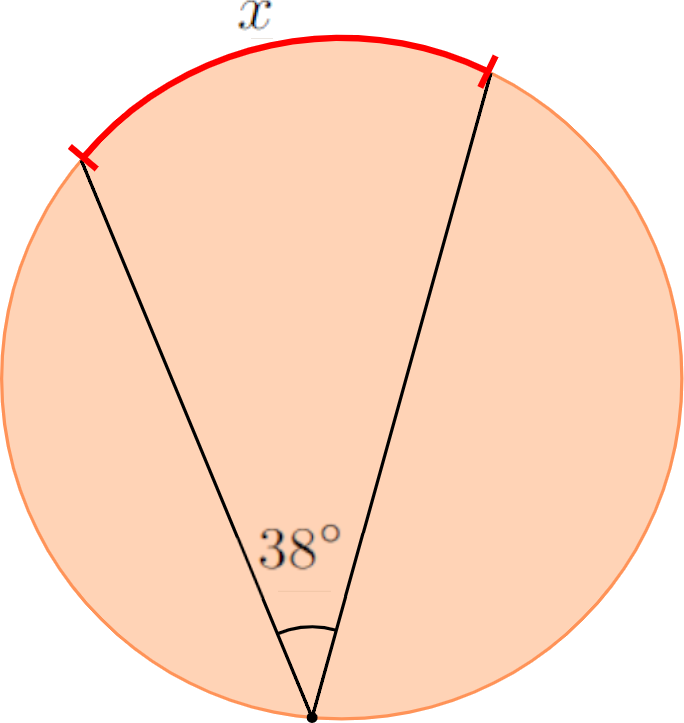
\includegraphics[width=0.7\linewidth]{mex_0054.png}\\
                $x=$ \fillin[$$ u][0.4in]

                \part 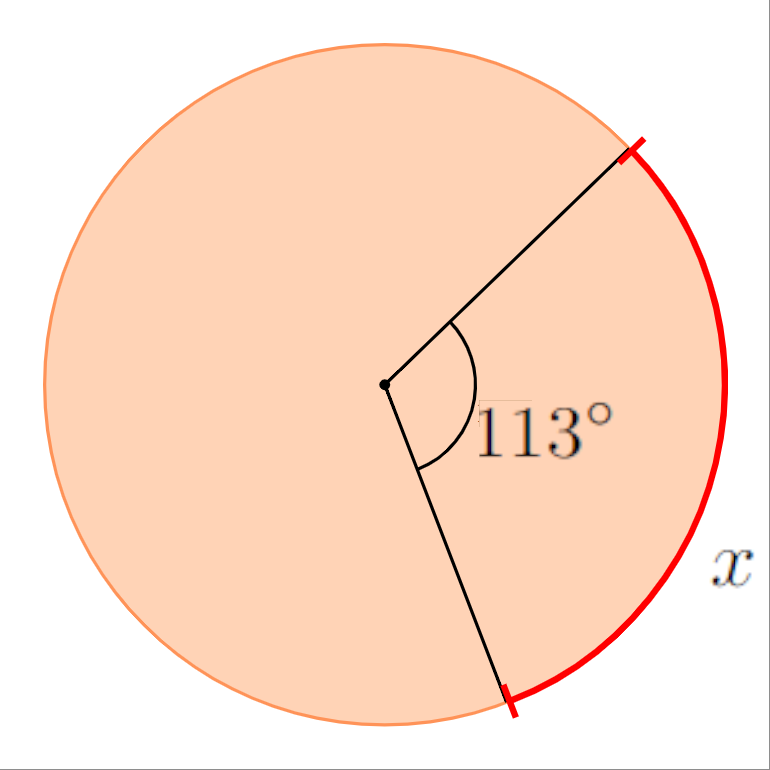
\includegraphics[width=0.7\linewidth]{mex_0055.png}\\
                $x=$ \fillin[$$ u][0.4in]

                \part 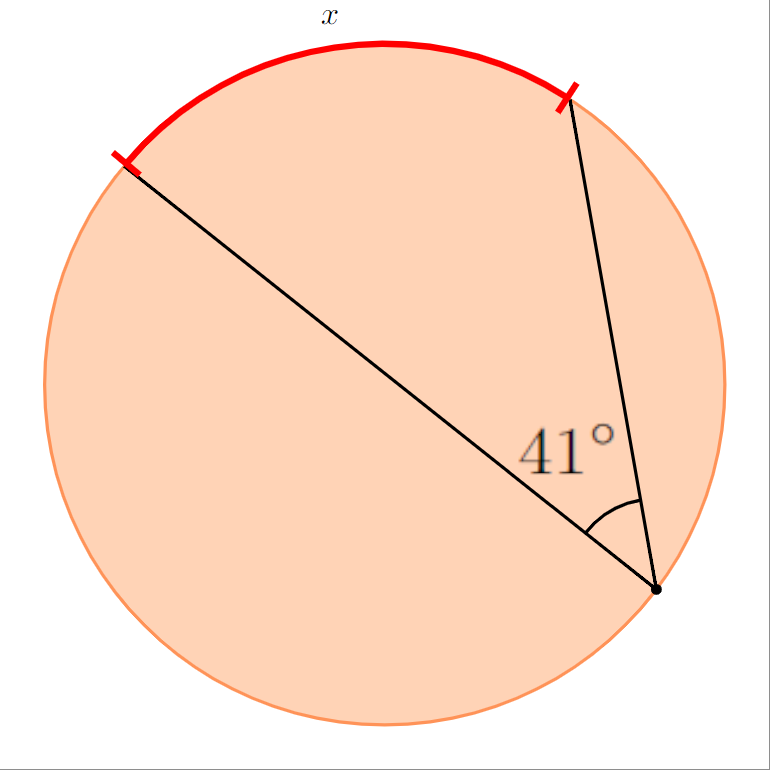
\includegraphics[width=0.7\linewidth]{mex_0056.png}\\
                $x=$ \fillin[$$ u][0.4in]

                \part 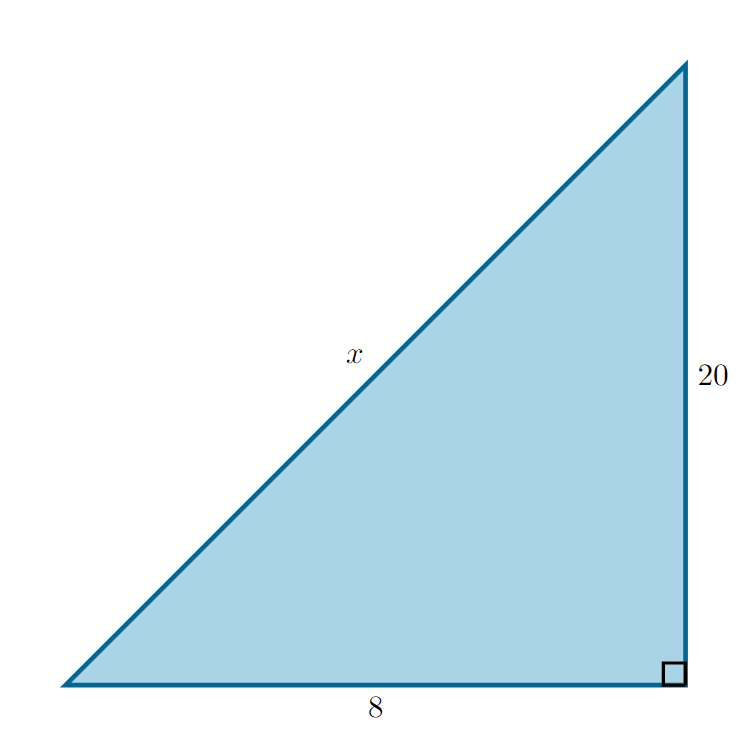
\includegraphics[width=0.7\linewidth]{mex_0057.png}\\
                $x=$ \fillin[$$ u][0.4in]
            \end{parts}
        \end{multicols}
    }

    \subsection*{Área de un sector circular}

    \questionboxed[6]{Calcula el área de cada uno de los siguientes sectores circulares:
        \begin{multicols}{2}
            \begin{parts}
                \part 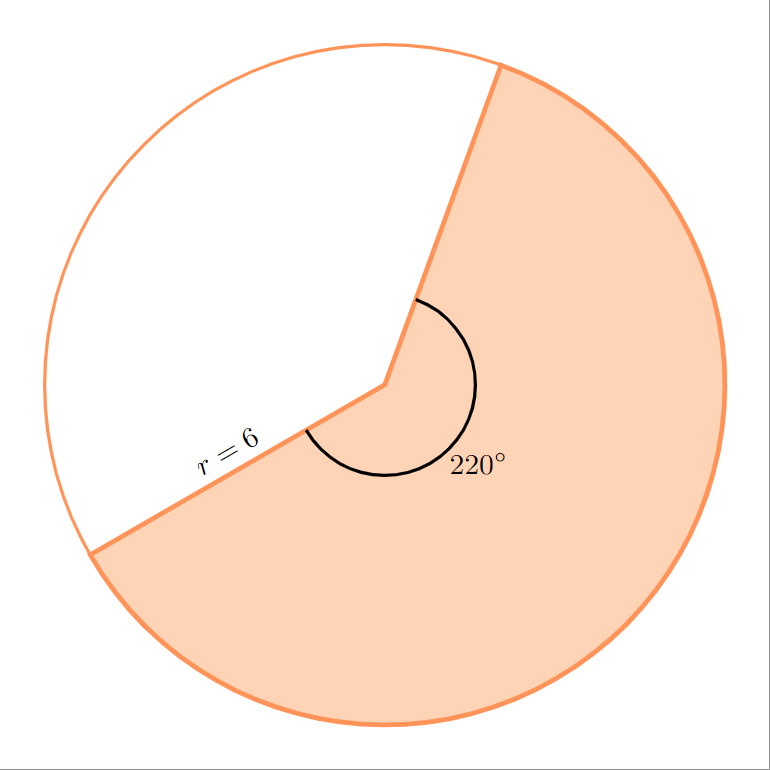
\includegraphics[width=0.7\linewidth]{mex_0058.png}\\
                Área= \fillin[$$ u][0.4in]

                \part 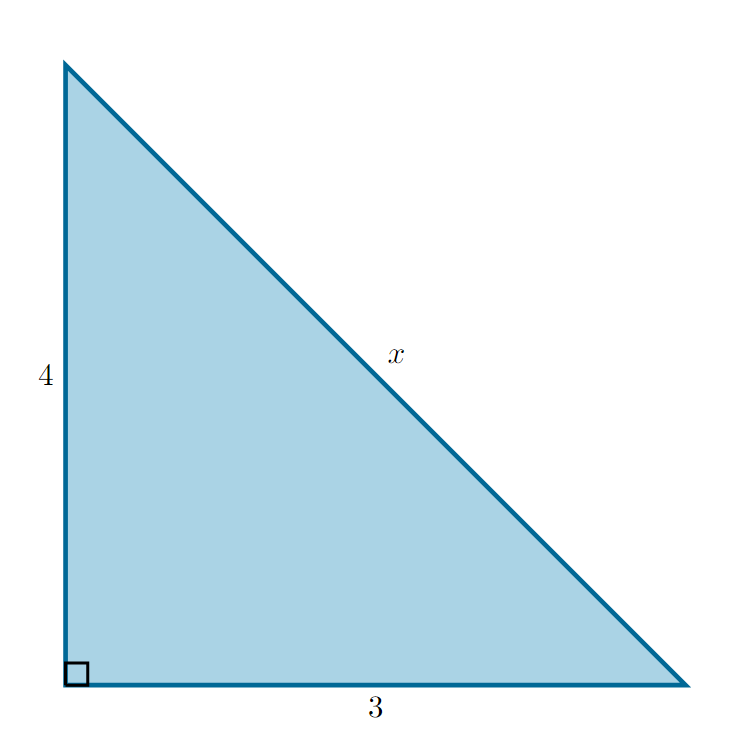
\includegraphics[width=0.7\linewidth]{mex_0059.png}\\
                Área= \fillin[$$ u][0.4in]

                \part 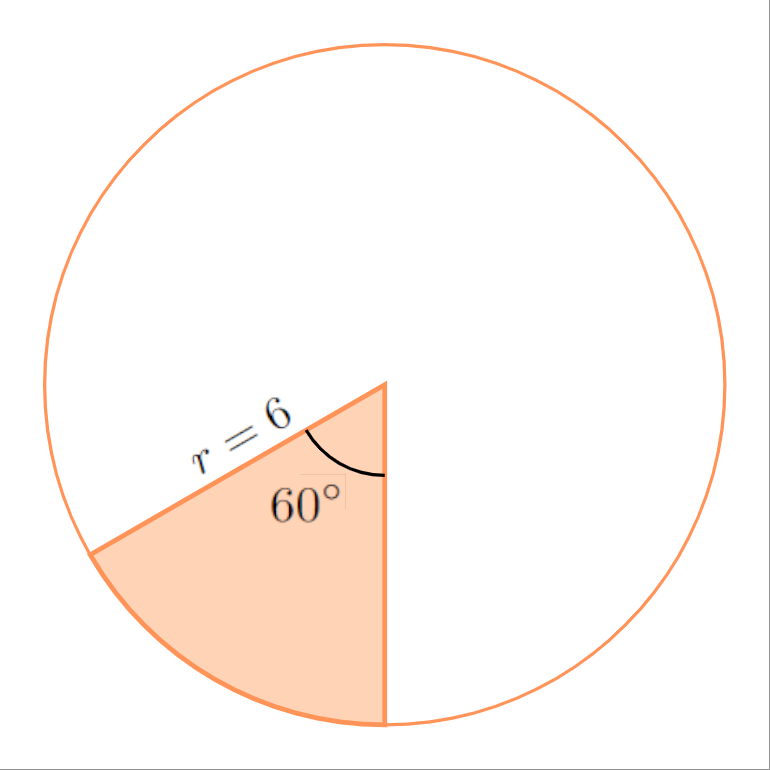
\includegraphics[width=0.7\linewidth]{mex_0060.png}\\
                Área= \fillin[$$ u][0.4in]

                \part 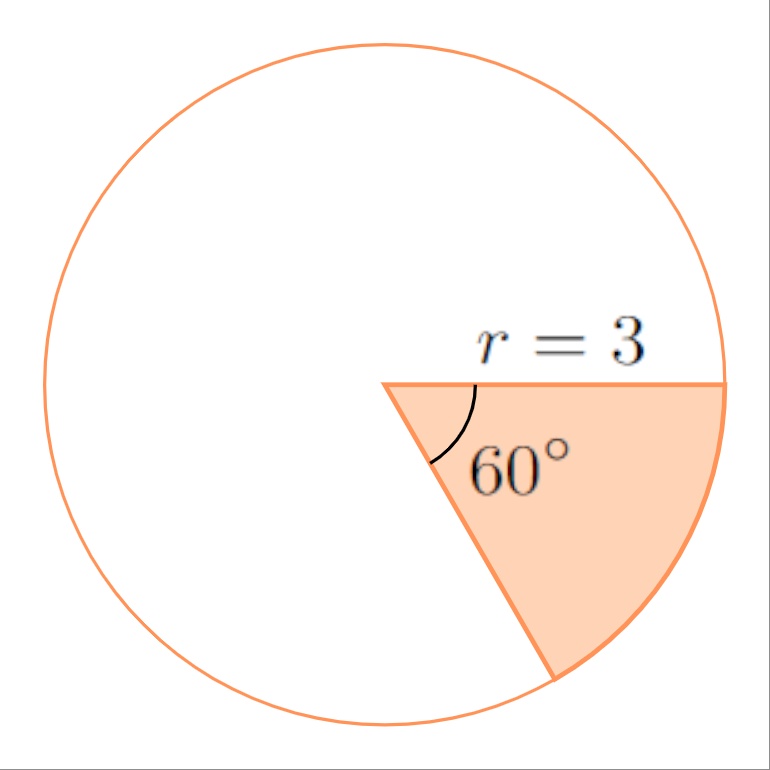
\includegraphics[width=0.7\linewidth]{mex_0061.png}\\
                Área= \fillin[$$ u][0.4in]

                \part 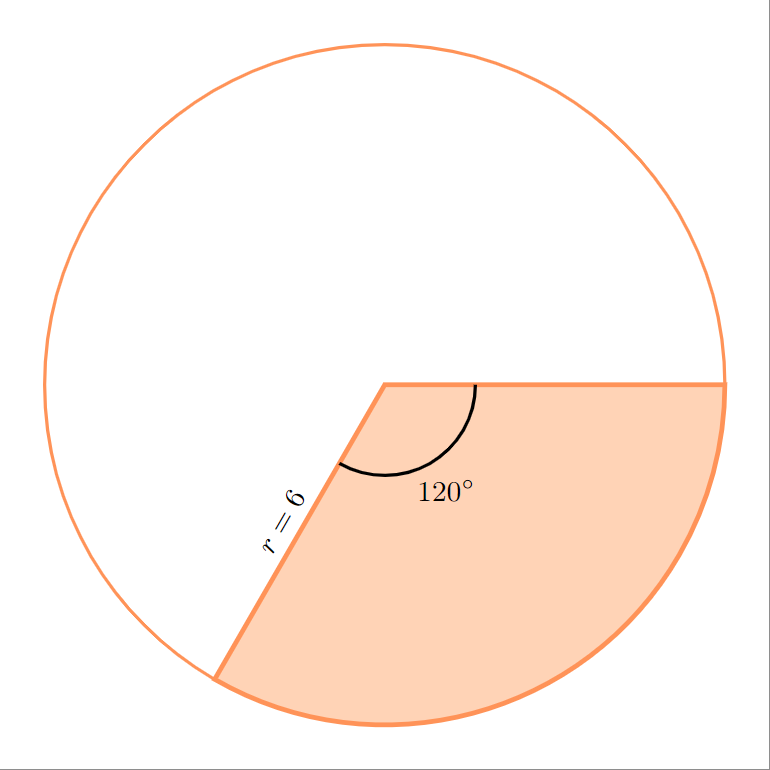
\includegraphics[width=0.7\linewidth]{mex_0062.png}\\
                Área= \fillin[$$ u][0.4in]

                \part 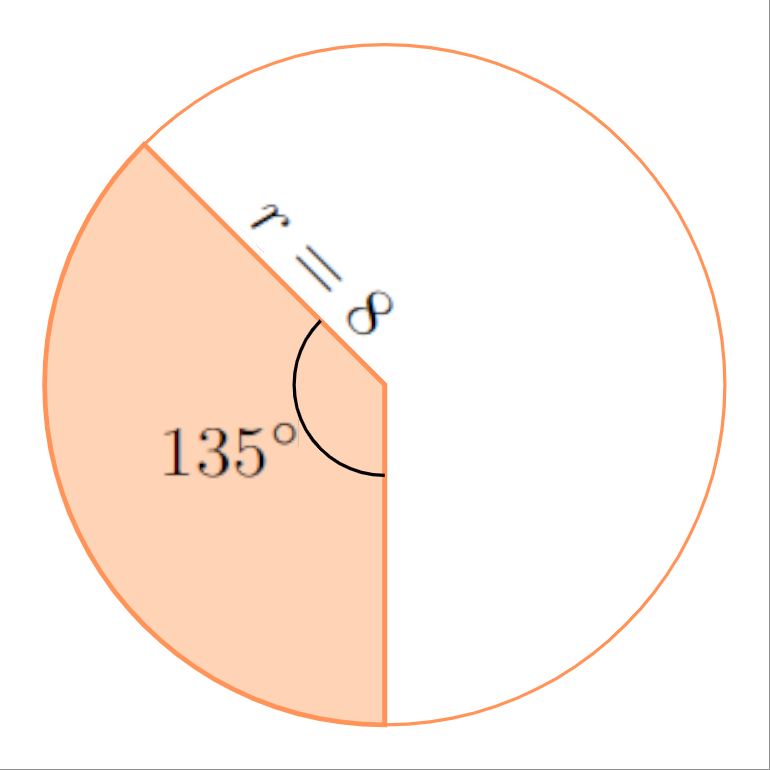
\includegraphics[width=0.7\linewidth]{mex_0063.png}\\
                Área= \fillin[$$ u][0.4in]
            \end{parts}
        \end{multicols}
    }

    \section*{Figuras y cuerpos geométricos}
    \subsection*{Perímetro y Área}
    \questionboxed[4]{Encuentra el perímetro y el área de las siguientes figuras:
        \begin{multicols}{2}
            \begin{parts}
                % \part 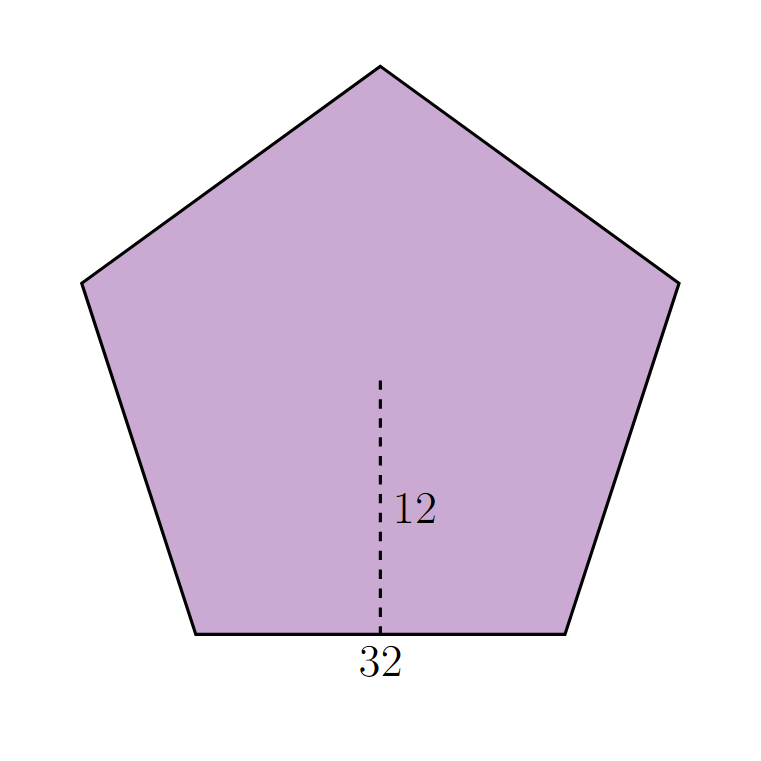
\includegraphics[width=\linewidth]{mex_0018.png}
                % Perímetro: \fillin[$$ u][0.4in] \qquad Área: \fillin[$$ u$^2$][0.4in]

                \part 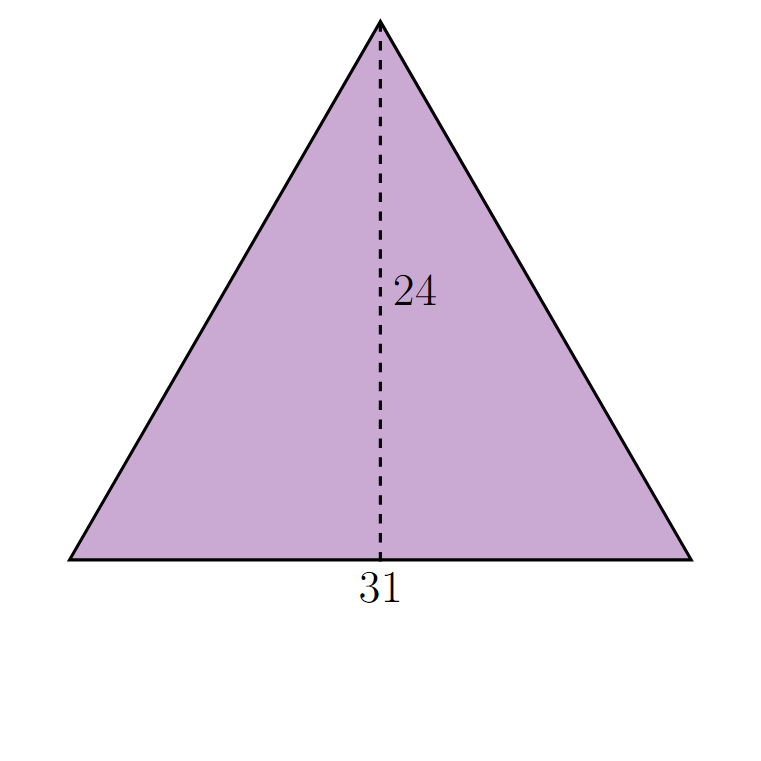
\includegraphics[width=0.6\linewidth]{mex_0017.png}\\
                Perímetro: \fillin[$$ u][0.4in] \qquad Área: \fillin[$$ u$^2$][0.4in]

                % \part 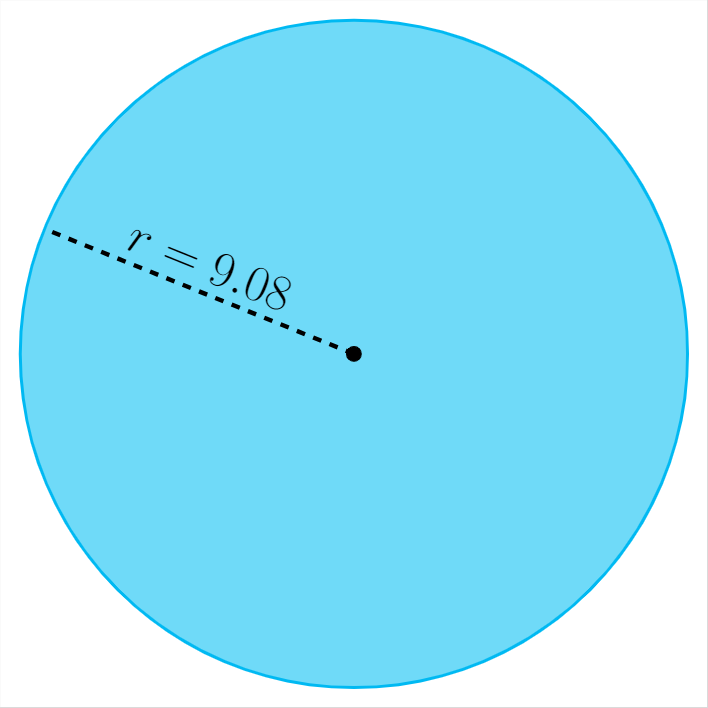
\includegraphics[width=\linewidth]{mex_0012.png}
                % Perímetro: \fillin[$$ u][0.4in] \qquad Área: \fillin[$$ u$^2$][0.4in]

                \part 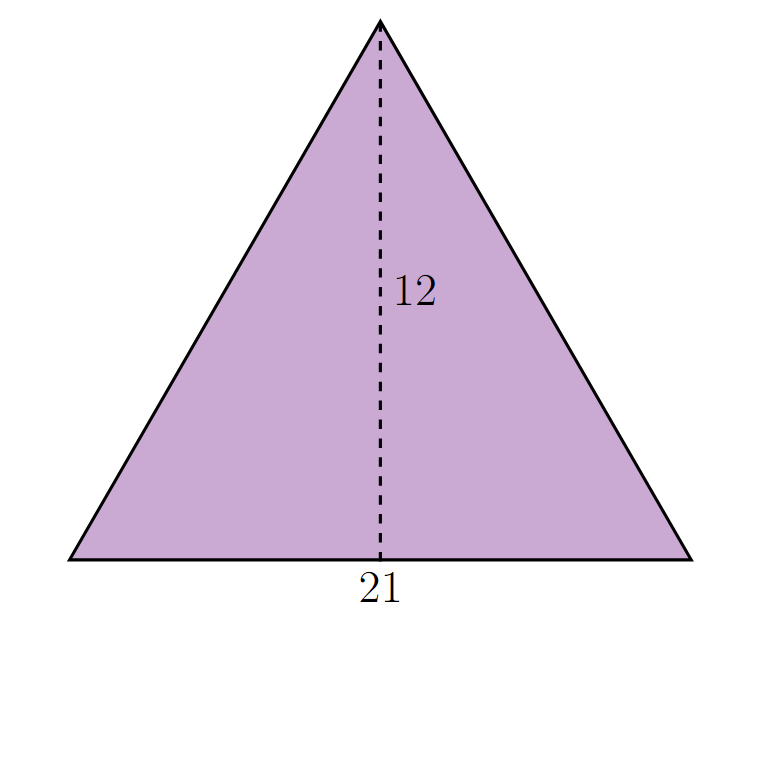
\includegraphics[width=0.6\linewidth]{mex_0020.png}\\
                Perímetro: \fillin[$$ u][0.4in] \qquad Área: \fillin[$$ u$^2$][0.4in]

                \part 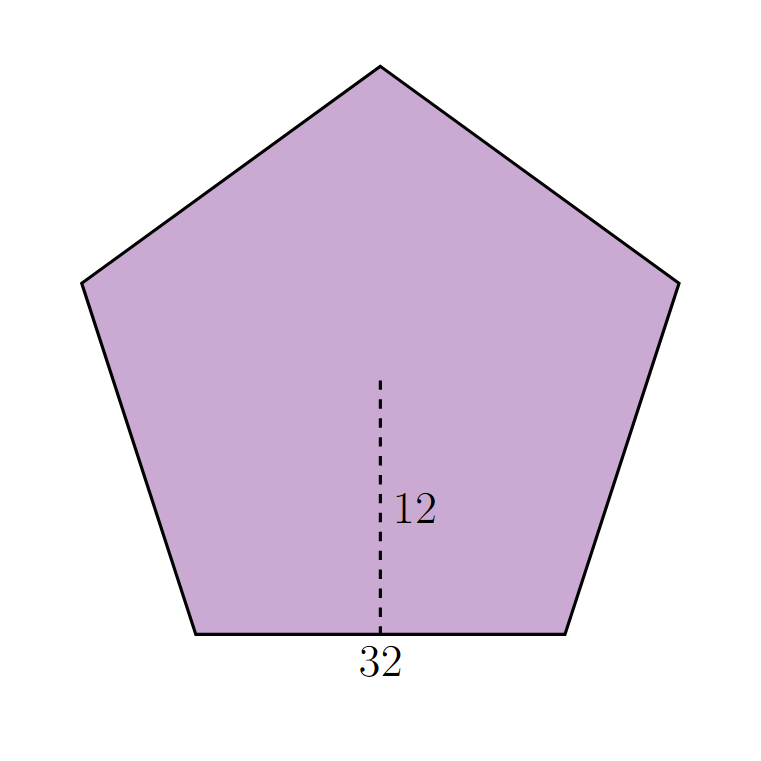
\includegraphics[width=0.6\linewidth]{mex_0018.png}\\
                Perímetro: \fillin[$$ u][0.4in] \qquad Área: \fillin[$$ u$^2$][0.4in]

                % \part 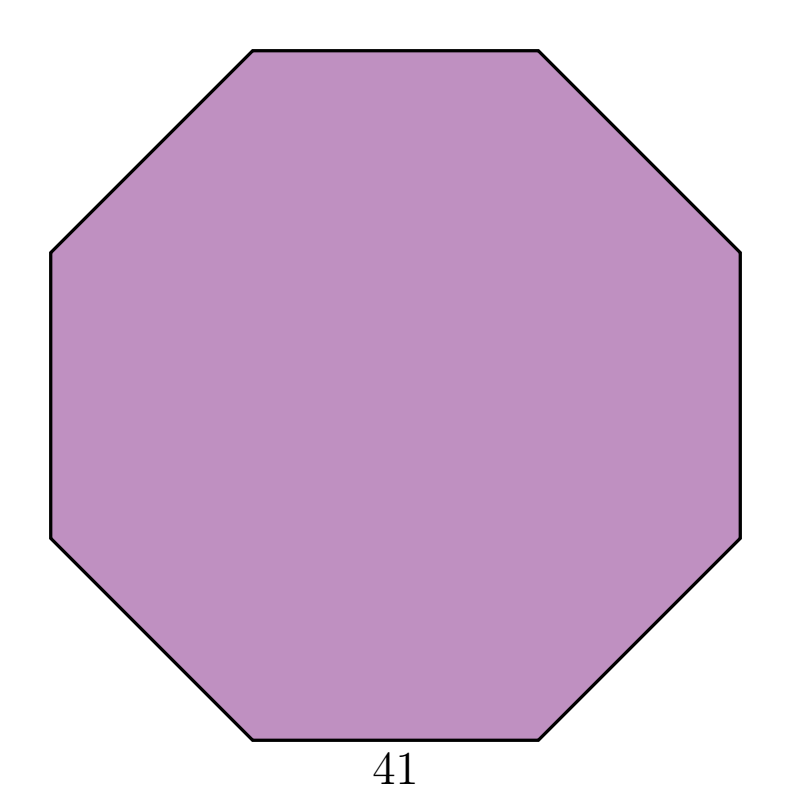
\includegraphics[width=\linewidth]{mex_0005.png}
                % Perímetro: \fillin[$$ u][0.4in] \qquad Área: \fillin[$$ u$^2$][0.4in]

                % \part 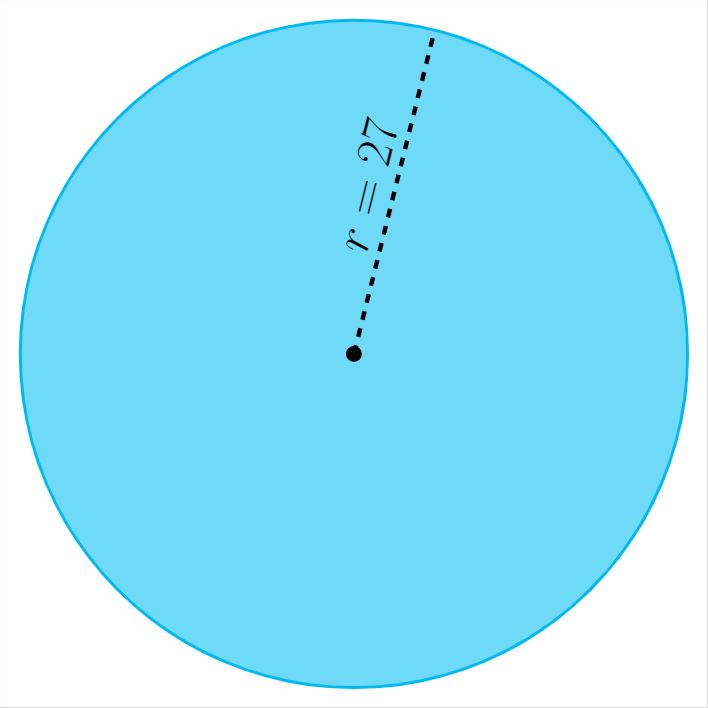
\includegraphics[width=\linewidth]{mex_0006.png}
                % Perímetro: \fillin[$$ u][0.4in] \qquad Área: \fillin[$$ u$^2$][0.4in]

                % \part 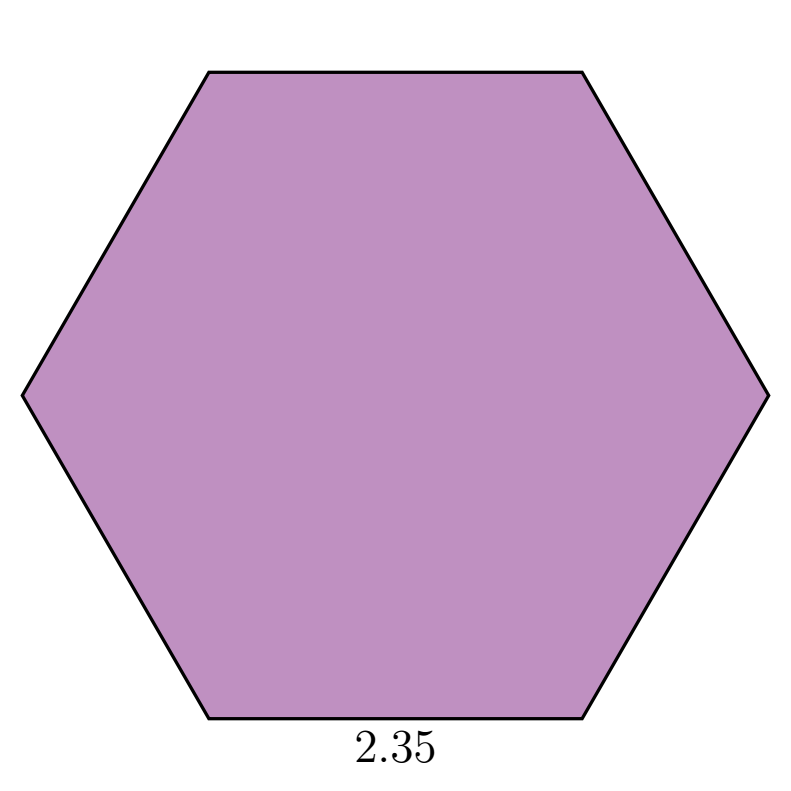
\includegraphics[width=\linewidth]{mex_0007.png}
                % Perímetro: \fillin[$$ u][0.4in] \qquad Área: \fillin[$$ u$^2$][0.4in]

                \part 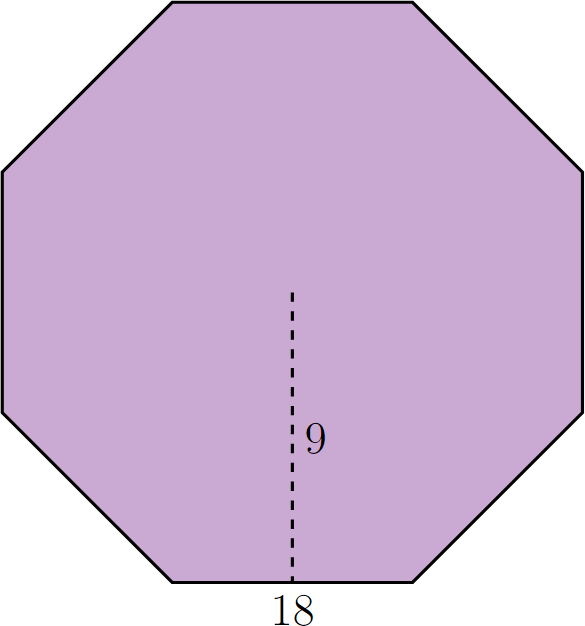
\includegraphics[width=0.6\linewidth]{mex_0016.png}\\
                Perímetro: \fillin[$$ u][0.4in] \qquad Área: \fillin[$$ u$^2$][0.4in]

            \end{parts}
        \end{multicols}
    }

    \subsection*{Resolución de problemas}
    \questionboxed[4]{Resuelve los siguientes problemas:
        \begin{multicols}{2}
            \begin{parts}
                \part Ricardo quiere poner una barda alrededor de un terreno pentagonal que mide 15 metros por lado. ¿Cuánta barda necesitará Ricardo para poner barda en todo el terreno?

                \begin{solutionbox}{1cm}
                \end{solutionbox}

                \part Calcula la altura de un prisma que tiene como área de la base 6 m$^2$ y 66 m$^3$ de capacidad.

                \begin{solutionbox}{1cm}
                \end{solutionbox}

                \part Calcula la altura de un prisma que tiene como área de la base 8 m$^2$ y 120 m$^3$ de capacidad.

                \begin{solutionbox}{1cm}
                \end{solutionbox}

                \part ¿Cuál es el perímetro de un campo de fútbol que mide 95.12 metros de largo y 45.27 metros de ancho?

                \begin{solutionbox}{1cm}
                \end{solutionbox}
            \end{parts}
        \end{multicols}
    }

    \subsection*{Área lateral, Área total y Volumen}
    \questionboxed[4]{Calcula el volumen, el área lateral y el área total de las siguientes figuras:
        \begin{multicols}{2}
            \begin{parts}
                \part 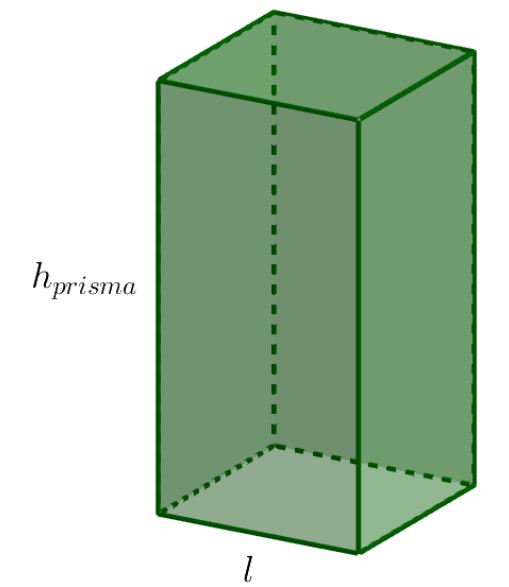
\includegraphics[width=0.8\linewidth]{mex_0026.png}\\
                Prisma cuyos lados "l" de la base miden 8 cm y la altura "h" mide 21 cm.\\
                Volumen: \fillin[$1344$ cm$^3$][0.4in] \\A. Lateral: \fillin[$672$ cm$^2$][0.4in] \\ A. Total: \fillin[$800$ cm$^2$][0.4in]

                % \part 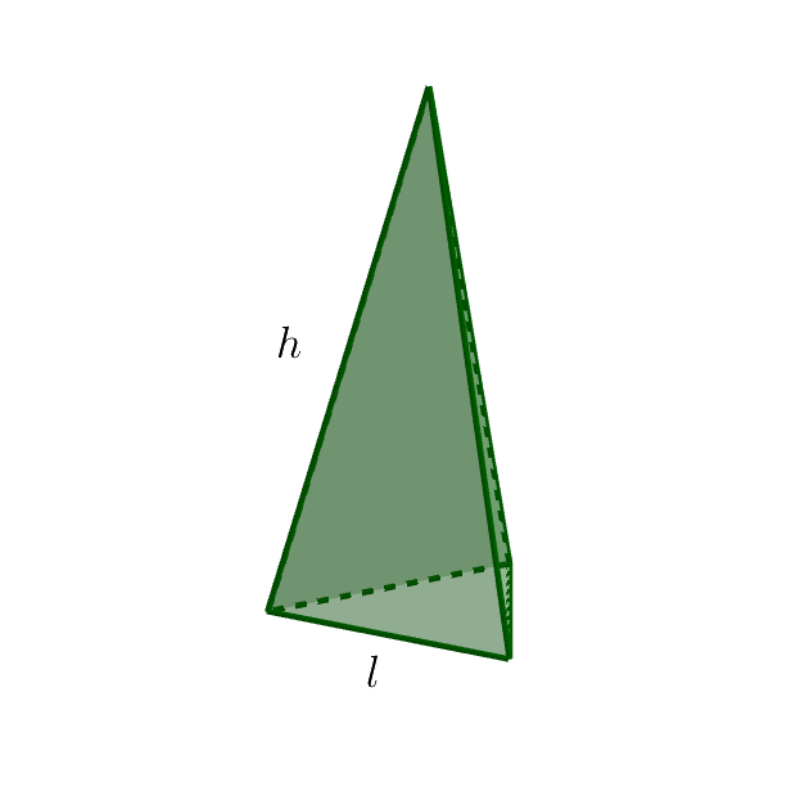
\includegraphics[width=\linewidth]{mex_0023.png}
                % Pirámide cuyos lados "l" de la base miden 13 cm y la altura "h" mide 42 cm.\\
                % Volumen: \fillin[$$ u$^3$][0.4in] \\A. Lateral: \fillin[$$ u][0.4in] \\ A. Total: \fillin[$$ u$^2$][0.4in]

                \part 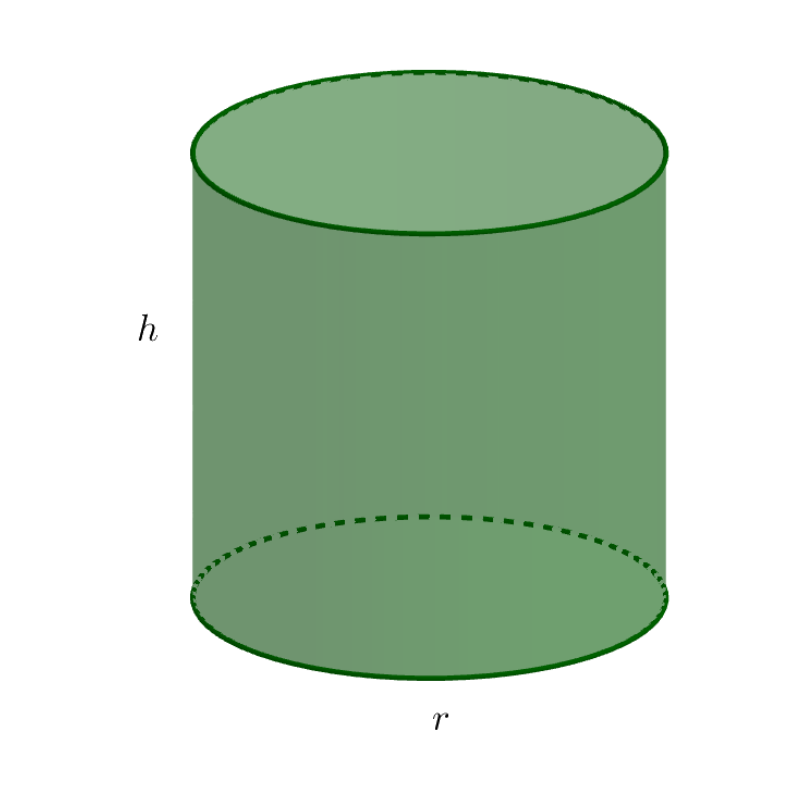
\includegraphics[width=0.8\linewidth]{mex_0024.png}\\
                Cilindro con altura $h=17$ cm y un radio $r=4$ cm.\\
                Volumen: \fillin[$854.08$ cm$^3$][0.4in] \\A. Lateral: \fillin[$100.48$ cm$^2$][0.4in] \\ A. Total: \fillin[$527.52$ cm$^2$][0.4in]

                \part 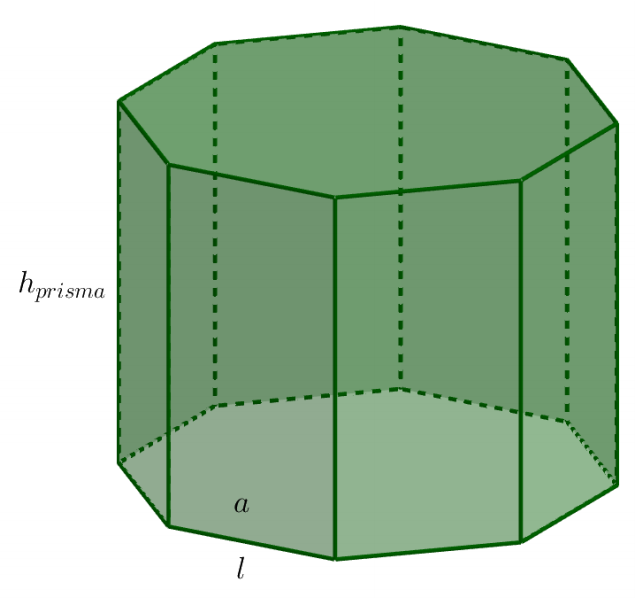
\includegraphics[width=0.8\linewidth]{mex_0025.png}\\
                Prisma de 19 cm de altura  y su base es un octágono cuyos los lados "l" miden 7 cm y tiene una apotema "a" de 5 cm.\\
                Volumen: \fillin[$2660$ cm$^3$][0.4in] \\A. Lateral: \fillin[$1064$ u][0.4in] \\ A. Total: \fillin[$1344$ cm$^2$][0.4in]

                % \part 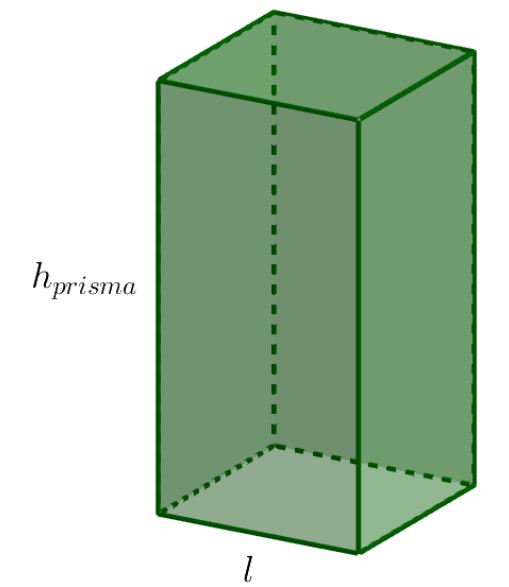
\includegraphics[width=0.8\linewidth]{mex_0026.png}\\
                % Prisma cuyos lados "l" de la base miden 15 cm y la altura "h" mide 24 cm.\\
                % Volumen: \fillin[$$ u$^3$][0.4in] \\A. Lateral: \fillin[$$ u][0.4in] \\ A. Total: \fillin[$$ u$^2$][0.4in]

                % \part 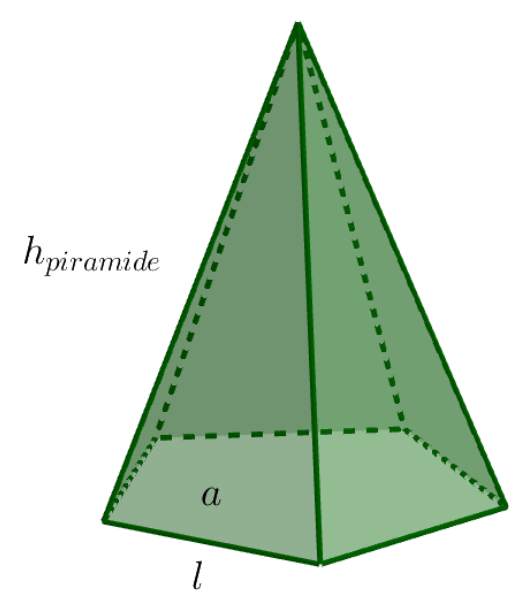
\includegraphics[width=0.8\linewidth]{mex_0027.png}\\
                % Pirámide de 19 cm de altura cuya base es un pentágono cuyos lados "l" miden 8 cm y su apotema "a" mide 5 cm.\\
                % Volumen: \fillin[$$ u$^3$][0.4in] \\A. Lateral: \fillin[$$ u][0.4in] \\ A. Total: \fillin[$$ u$^2$][0.4in]

                \part 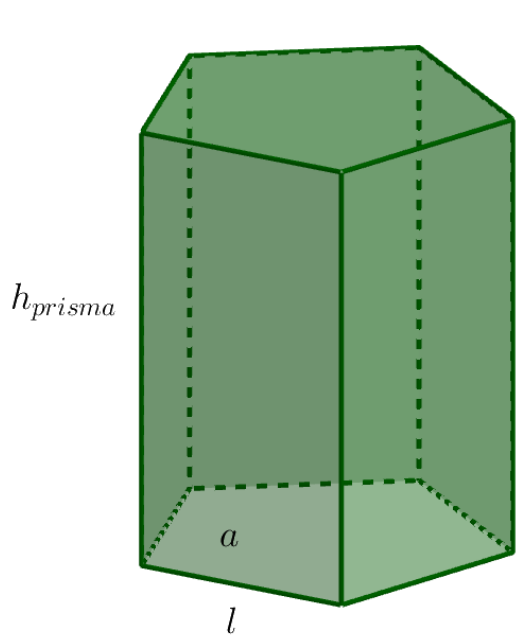
\includegraphics[width=0.8\linewidth]{mex_0028.png}\\
                Prisma de 32 cm de altura  y su base es un pentágono cuyos los lados "l" miden 13 cm y tiene una apotema "a" de 8 cm.\\
                Volumen: \fillin[$8320$ cm$^3$][0.4in] \\A. Lateral: \fillin[$2080$ cm$^2$][0.4in] \\ A. Total: \fillin[$2600$ cm$^2$][0.4in]

                % \part 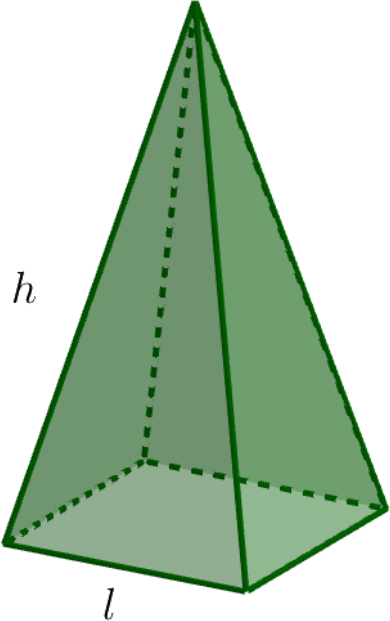
\includegraphics[width=0.8\linewidth]{mex_0029.png}\\
                % Pirámide cuyos lados "l" de la base miden 16 cm y la altura "h" mide 27 cm.\\
                % Volumen: \fillin[$$ u$^3$][0.4in] \\A. Lateral: \fillin[$$ u][0.4in] \\ A. Total: \fillin[$$ u$^2$][0.4in]

                % \part 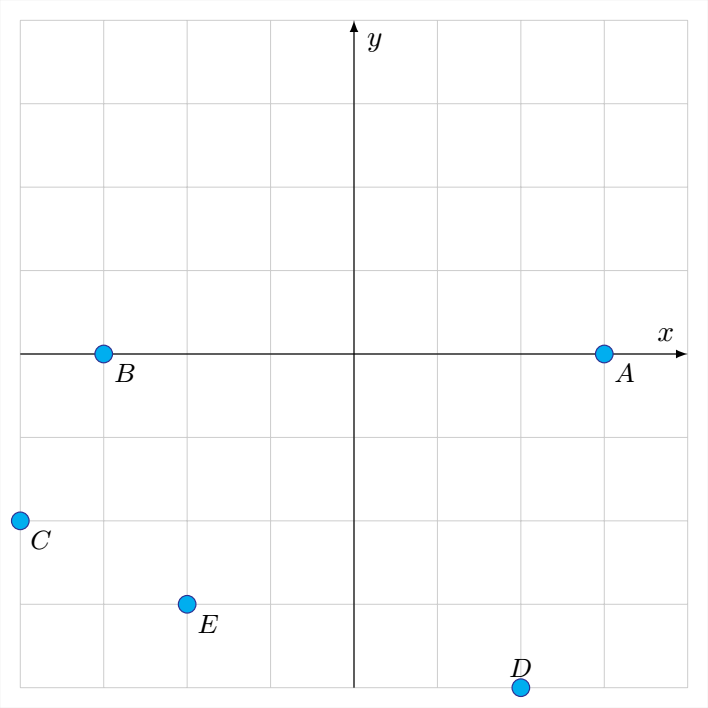
\includegraphics[width=\linewidth]{mex_0030.png}
                % Volumen: \fillin[$$ u$^3$][0.4in] \\A. Lateral: \fillin[$$ u][0.4in] \\ A. Total: \fillin[$$ u$^2$][0.4in]

            \end{parts}
        \end{multicols}
    }

    \newpage
    \section*{Monomios y polinomios}
    \subsection*{Lenguaje algebraico}

    \questionboxed[4]{Elige la expresión algebraica correcta para cada uno de los siguientes enunciados:

        \begin{multicols}{2}
            \begin{parts}
                \part A un número se le resta 14.

                \begin{oneparchoices}
                    \choice $a+14$
                    \CorrectChoice $a-14$
                    \choice $14a$
                    \choice $\dfrac{a}{14}$
                \end{oneparchoices}

                \part La suma de tres número diferentes

                \begin{oneparchoices}
                    \choice $-xyz$
                    \choice $xyz$
                    \CorrectChoice $x+y+z$
                    \choice $x+y-z$
                \end{oneparchoices}

                \part El cubo de un número aumentado en 10

                \begin{oneparchoices}
                    \choice $3x+10$
                    \choice $(x+10)^3$
                    \CorrectChoice $x^3+10$
                    \choice $x+10$
                \end{oneparchoices}

                \part El doble de la suma de un n\'umero con 2


                \begin{oneparchoices}
                    \CorrectChoice $2(x+2)$
                    \choice $2x+2$
                    \choice $2+x$
                    \choice $(x+2)^2$
                \end{oneparchoices}

                \part La diferencia del triple de un n\'umero con 1.


                \begin{oneparchoices}
                    \choice $3(1-a)$
                    \choice $3a+1$
                    \CorrectChoice $1-3a$
                    \choice $\dfrac{1}{3a}$
                \end{oneparchoices}

                \part Cinco novenos del cuadrado de un n\'umero.

                \begin{oneparchoices}
                    \choice $\left(\dfrac{5}{9}x\right)^2$
                    \choice $\left(\dfrac{9}{5}x\right)^2$
                    \choice $5(9x^2)$
                    \CorrectChoice $\dfrac{5}{9}x^2$
                \end{oneparchoices}

                \part La mitad de la suma de un n\'umero con 3.


                \begin{oneparchoices}
                    \choice $\frac{1}{2}x+3$
                    \CorrectChoice $\frac{x+3}{2}$
                    \choice $\frac{1}{2}+x+3$
                    \choice $\frac{x}{2}+3$
                \end{oneparchoices}

                \part La suma de la mitad de un n\'umero con 3.


                \begin{oneparchoices}
                    \CorrectChoice $\frac{1}{2}x+3$
                    \choice $\frac{x+3}{2}$
                    \choice $\frac{1}{2}+x+3$
                    \choice $\frac{x}{2}+3$
                \end{oneparchoices}


            \end{parts}
        \end{multicols}
    }

    \subsection*{Suma de monomios y polinomios}

    \questionboxed[4]{Resuelve las siguientes sumas de monomios y polinomios:

        \begin{multicols}{2}
            \begin{parts}
                \part $12x+8x+50x=$ \fillin[$70x$][0in]
                \part $(a+3b)+(2a+4b)+(-8a-10b)=$ \fillin[$-5a-3b$][0in]
                \part $(5m-9n+5p)+(2m-n-4p)+(m+n-4p)=$ \fillin[$8m-9n-3p$][0in]
                \part $(b+9c)+(-2b-3c)+(2a-4b-5c)=$ \fillin[$2a-5b+c$][0in]
                \part $(4x-y+3z)+(-4x+y-3z)=$ \fillin[$0$][0in]
                \part $18n+13n+19n=$ \fillin[$50n$][0in]
                \part $(a-4b+3c)+(2a+4b-c)+(3a-2b+4c)=$ \fillin[$6a-2b+6c$][0in]
                \part $(a+b+c)+(2a+2b+2c)=$ \fillin[$3a+3b+3c$][0in]
            \end{parts}
        \end{multicols}
    }

    \subsection*{Resta de monomios y polinomios}

    \questionboxed[4]{Resuelve las siguientes sumas de monomios y polinomios:

        \begin{multicols}{2}
            \begin{parts}
                \part $a-2a-3a=$ \fillin[$-4a$][0in]
                \part $(8a-b-5c)-(-2a+5b+3c)=$ \fillin[$10a-6b-8c$][0in]
                \part $(5x-2y)-(2y-z)-(7x+3y-4z)=$ \fillin[$-2x-7y+5z$][0in]
                \part $(4x-3y-z)-(2x-5y+3z)=$ \fillin[$2x+2y-4z$][0in]
                \part $(a+2b+3c)-(a-b+c)-(3a-4b-c)=$ \fillin[$-3a+7b+3c$][0in]
                \part $(x+y+z)-(4x-5y+3z=$ \fillin[$-3x+6y-2z$][0in]
                \part $(3x-5y+4z)-(2x+5y+4z)=$ \fillin[$x-10y$][0in]
                \part $18x-22x-10x=$ \fillin[$-14x$][0in]
            \end{parts}
        \end{multicols}
    }

    \subsection*{Operaciones combinadas}

    \questionboxed[4]{Resuelve las siguientes operaciones convinadas:
        \begin{multicols}{2}
            \begin{parts}
                \part $-5(3x+5)+4(7x-2)=$ \fillin[$13x-33$][0in]
                \part $-5(5y+2)+3(-9y)=$ \fillin[$-52y-10$][0in]
                \part $3(10x-5y+2)+2(6x-9y)=$ \fillin[$42x-33y+6$][0in]
                \part $2(x-3y+7)-5(3x+4y-7)=$ \fillin[$-13x-26y+49$][0in]
                \part $(x-7y+2)-3(2x-3y+4)=$ \fillin[$-5x+2y-10$][0in]
                \part $2(8x)+5(-x+7)=$ \fillin[$11x+35$][0in]
                \part $3(x+y-5)+5(2x-3y+1)-3(4x-y-3)=$ \fillin[$x-9y-1$][0in]
                \part $3(5x+3)-2(-2x+3)+4(2x-6)=$ \fillin[$27x-21$][0in]
            \end{parts}
        \end{multicols}
    }

    \subsection*{Perímetro de figuras geométricas}

    \questionboxed[3]{Encuentra el perímetro de las siguientes figuras:
        \begin{multicols}{3}
            \begin{parts}
                \part 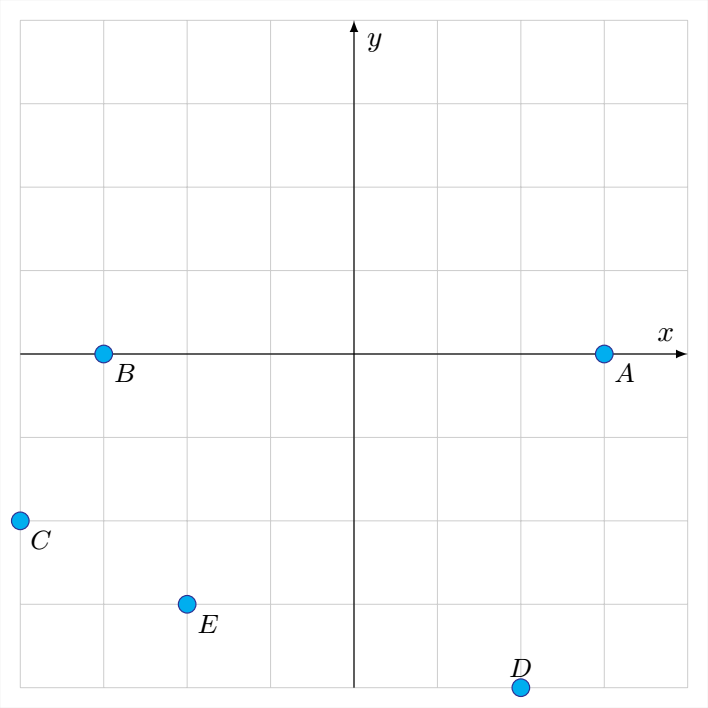
\includegraphics[width=\linewidth]{mex_0030.png}\\
                Perímetro: \fillin[$40x-24y$][1in]
                \part 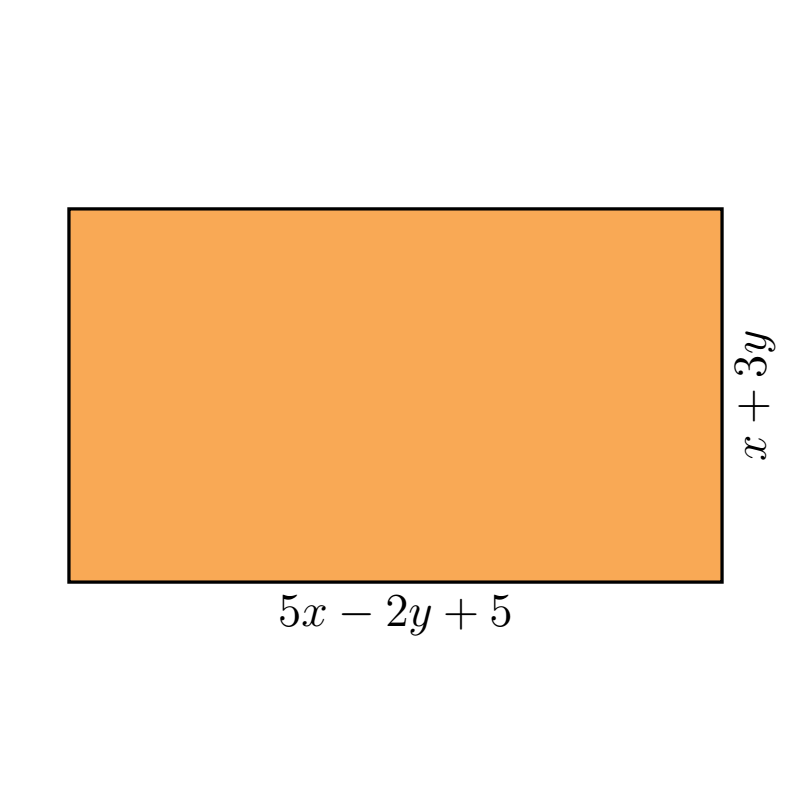
\includegraphics[width=\linewidth]{mex_0031.png}\\
                Perímetro: \fillin[$12x+2y+10$][1in]
                \part \includegraphics[width=\linewidth]{mex_0032.png}\\
                Perímetro: \fillin[$12a-18b-30$][1in]
                \part \includegraphics[width=\linewidth]{mex_0033.png}\\
                Perímetro: \fillin[$24x+48y-8$][1in]
                \part \includegraphics[width=\linewidth]{mex_0034.png}\\
                Perímetro: \fillin[$6x+8y-12$][1in]
                \part \includegraphics[width=\linewidth]{mex_0035.png}\\
                Perímetro: \fillin[$12x+4y-8$][1in]
            \end{parts}
        \end{multicols}
    }

    \newpage
    \section*{Operaciones con monomios y polinomios}
    \subsection*{Suma, resta y multiplicación de exponentes}

    \questionboxed[6]{Realiza las siguientes operaciones con exponentes:
        \begin{multicols}{3}
            \begin{parts}
                \subsection*{\ifprintanswers{Suma de exponentes}\else{}\fi}
                \part $(-5a^4)(-3a^2)=$ \fillin[$15a^6$][0in]
                \begin{solutionbox}{2cm}
                    $(-5a^4)(-3a^2) = 15a^6$
                \end{solutionbox}

                \part $(-3a^4)(8a^2)=$
                \begin{solutionbox}{2cm}
                    $(-3a^4)(8a^2) = -24a^6$
                \end{solutionbox}

                \part $4x^2\cdot x^5\cdot 5x^8=$
                \begin{solutionbox}{2cm}
                    $4x^2\cdot x^5\cdot 5x^8 = 20x^{15}$
                \end{solutionbox}

                \part $x^2y^3z^4 \cdot x^5z^4=$
                \begin{solutionbox}{2cm}
                    $x^2y^3z^4 \cdot x^5z^4 = x^7y^3z^8$
                \end{solutionbox}

                \columnbreak

                \part $x^3x^2x^3=$
                \begin{solutionbox}{2cm}
                    $x^3x^2x^3 = x^8$
                \end{solutionbox}

                \part $7x^2\cdot 3x^4 \cdot 6x^2=$
                \begin{solutionbox}{2cm}
                    $7x^2\cdot 3x^4 \cdot 6x^2 = 126x^8$
                \end{solutionbox}

                \subsection*{\ifprintanswers{Resta de exponentes}\else{}\fi}
                \part $\dfrac{x^{13}y^{18}z^{4}}{x^{11}y^{9}z^{4}}=$ \fillin[$x^2y^9$][0in]
                \begin{solutionbox}{2cm}
                    $\dfrac{x^{13}y^{18}z^{4}}{x^{11}y^{9}z^{4}} = x^2y^9$
                \end{solutionbox}

                \part $\dfrac{x^{4}y^{12}z^{13}}{x^{3}y^{12}z^{13}}=$
                \begin{solutionbox}{2cm}
                    $\dfrac{x^{4}y^{12}z^{13}}{x^{3}y^{12}z^{13}} = x$
                \end{solutionbox}

                \part $\dfrac{81a^5b^{12}c^9}{9a^3b^{7}c^5}=$
                \begin{solutionbox}{2cm}
                    $\dfrac{81a^5b^{12}c^9}{9a^3b^{7}c^5} = 9a^2b^5c^4$
                \end{solutionbox}

                \subsection*{\ifprintanswers{Multiplicación de exponentes}\else{}\fi}
                \part $(a^3b^2c^4)^3=$ \fillin[$a^9b^6c^{12}$][0in]
                \begin{solutionbox}{2cm}
                    $(a^3b^2c^4)^3 = a^9b^6c^{12}$
                \end{solutionbox}

                \part $\left(x^4 y^5\right)^6=$
                \begin{solutionbox}{2cm}
                    $\left(x^4 y^5\right)^6 = x^{24}y^{30}$
                \end{solutionbox}

                \part $\left(a^3 b^5 c^{11} \right)^7=$
                \begin{solutionbox}{2cm}
                    $\left(a^3 b^5 c^{11} \right)^7 = a^{21}b^{35}c^{77}$
                \end{solutionbox}
            \end{parts}
        \end{multicols}
    }

    \subsection*{Multiplicación y división de monomios y polinomios}

    \questionboxed[4]{Realiza la siguientes multiplicaciones de polinomios:
        \begin{multicols}{2}
            \begin{parts}
                \part $(x-3)(x^2-5x+4)=$ \fillin[$x^3-8x^2+19x-12$][0in]
                \part $(2a+3b)(4x+3y)=$ \fillin[$8ax+6ay+12bx+9by$][0in]
                \part $(x+1)(x+2)(x+3)=$ \fillin[$x^3+6x^2+11x+6$][0in]
                \part $(x+5)(2x^2+3x-7)=$ \fillin[$2x^3+13x^2+8x-35$][0in]
                \part $(x-1)(x+1)(x^2+1)=$ \fillin[$x^4-1$][0in]
                \part $(x+5)(x^2+2x-3)=$ \fillin[$x^3+7x^2+7x-15$][0in]
                \part $(x+-3(x-3)(x-2)=$ \fillin[$x^3-8x^2+21x-18$][0in]
                \part $(x+y)(x^2-xy+y^2)=$ \fillin[$x^3+y^3$][0in]
            \end{parts}
        \end{multicols}
    }



    \subsection*{Áreas de figuras geométricas}

    \questionboxed[3]{Encuentra el área de las siguientes figuras:
        \begin{multicols}{2}
            \begin{parts}
                \part \includegraphics[width=0.8\linewidth]{mex_0036.png}\\
                Área: \fillin[$x^2-6x+9$][1in]
                \part \includegraphics[width=0.8\linewidth]{mex_0037.png}\\
                Área: \fillin[$10x^2-50x$][1in]
                \part \includegraphics[width=0.8\linewidth]{mex_0038.png}\\
                Área: \fillin[$x^2+7x-30$][1in]
                \part \includegraphics[width=0.8\linewidth]{mex_0039.png}\\
                Área: \fillin[$2x^2+4x$][1in]
                \part \includegraphics[width=0.8\linewidth]{mex_0040.png}\\
                Área: \fillin[$2x^2+11x+14$][1in]
                \part \includegraphics[width=0.8\linewidth]{mex_0041.png}\\
                Área: \fillin[$9x^2+12x+4$][1in]
            \end{parts}
        \end{multicols}
    }

    \section*{Sistema de unidades}
    \subsection*{Unidades de longitud}
    \questionboxed[5]{Convierte las siguientes unidades de longitud como se te pide:
        \begin{multicols}{2}
            \begin{parts}
                \part Convierte 4.9 kilómetros a metros.
                \part Convierte 34 metros a hectómetros
                \part Convierte 98 milímetros a centímetros
                \part Convierte 134 kilómetros a metros
                \part Convierte 134 centímetros a decámetros
            \end{parts}
        \end{multicols}
    }


    \subsection*{Unidades de masa}
    \questionboxed[5]{Convierte las siguientes unidades de masa como se te pide:
        \begin{multicols}{2}
            \begin{parts}
                \part Convierte 342 gramos a hectogramos.
                \part Convierte 8334 centigramos a gramos.
                \part Convierte 93.4 miligramos a centigramos.
                \part Convierte 29 decagramos a miligramos.
                \part Convierte 9 gramos a miligramos.
            \end{parts}
        \end{multicols}
    }

    \subsection*{Unidades de capacidad}
    \questionboxed[5]{Convierte las siguientes unidades de capacidad como se te pide:
        \begin{multicols}{2}
            \begin{parts}
                \part Convierte 27 hectolitros a decilitros.
                \part Convierte 8 mililitros a centilitros.
                \part Convierte 1094 mililitros a decilitros.
                \part Convierte 702 mililitros a decilitros.
                \part Convierte 19 litros a mililitros.
                \part Convierte 8200 litros a metros cúbicos.
                \part Convierte 4.8 decímetros cúbicos a litros.
                \part Convierte 750 litros a metros cúbicos.
                \part Convierte 567 milímetros cúbicos a litros.
                \part Convierte 4100 litros a metros cúbicos.
            \end{parts}
        \end{multicols}
    }
    \subsection*{Unidades de área y volumen}
    \questionboxed[5]{Convierte las siguientes unidades de área y volumen como se te pide:
        \begin{multicols}{2}
            \begin{parts}
                \part Convierte 8.03 metros cúbicos a milímetros cúbicos
                \part Convierte 8 kilómetros cuadrados a metros cuadrados
                \part Convierte 88 metros cuadrados a kilómetros cuadrados
                \part Convierte 18 decámetros cúbicos a milímetros cúbicos
                \part Convierte 801 milímetros cuadrados a decámetros cuadrados
            \end{parts}
        \end{multicols}
    }
\end{questions}
\end{document}